%%
%% Copyright 2022 OXFORD UNIVERSITY PRESS
%%
%% This file is part of the 'oup-authoring-template Bundle'.
%% ---------------------------------------------
%%
%% It may be distributed under the conditions of the LaTeX Project Public
%% License, either version 1.2 of this license or (at your option) any
%% later version.  The latest version of this license is in
%%    http://www.latex-project.org/lppl.txt
%% and version 1.2 or later is part of all distributions of LaTeX
%% version 1999/12/01 or later.
%%
%% The list of all files belonging to the 'oup-authoring-template Bundle' is
%% given in the file `manifest.txt'.
%%
%% Template article for OXFORD UNIVERSITY PRESS's document class `oup-authoring-template'
%% with bibliographic references
%%

%%%CONTEMPORARY%%%
\documentclass[a4paper,num-refs]{oup-contemporary}%

%%% Journal toggle; only specific options recognised.
%%% (Only "gigascience" and "general" are implemented now. Support for other journals is planned.)
\journal{gigascience}

\usepackage{graphicx}
\usepackage{siunitx}

%%% Flushend: You can add this package to automatically balance the final page, but if things go awry (e.g. section contents appearing out-of-order or entire blocks or paragraphs are coloured), remove it!
% \usepackage{flushend}

\graphicspath{{images/}}

% line numbers
%\usepackage[mathlines, switch]{lineno}
%\usepackage[right]{lineno}

% added commands and packages
\newtheorem{proof}{Proof}
\newtheorem{theorem}{Theorem}%  meant for continuous numbers
\newtheorem{proposition}[theorem]{Proposition}%
\newtheorem{example}{Example}%
\newtheorem{remark}{Remark}%
\newtheorem{definition}{Definition}
\newtheorem{assumption}{Assumption}
\newtheorem{proposition*}{Proposition}
\newcommand{\indep}{\perp \!\!\! \perp}
\newcommand{\eg}{\emph{e.g.}}
\usepackage{amsmath}
\usepackage{amssymb}
\usepackage{algorithm, algorithmicx, algpseudocode}
\DeclareMathOperator*{\argmin}{argmin} \def\mycitecolor{green!50!black}
\usepackage{mathtools}
\newcommand\myeq{\stackrel{\mathclap{\text{def}}}{=}}
\usepackage{booktabs} % For formal tables (eg. bottomrules command)
\usepackage{multirow} % For multirow in tables
\usepackage{threeparttable} % For table 
\usepackage{caption} % for subfigures
\usepackage{subcaption}
\usepackage{placeins} % for FloatBarrier command to prevent a figure to pass some point.
\usepackage{titlesec} % for title formatting
%\titleformat*{\subsection}{\color{jnlclr}\bfseries} % force colored subsection font for paragraphs
%\titleformat*{\paragraph}{\bfseries} % force bold font for paragraphs
\usepackage{algpseudocode} % for algorithmic

\bibliographystyle{unsrtnat}
% add external bibliography
%\usepackage[sorting=nyt,style=numeric,natbib=true,doi=false,isbn=false,url=false,eprint=false, maxnames=999, maxcitenames=2]{biblatex} 
%\let\cite=\supercite
%\DeclareNameAlias{default}{last-first}
%\addbibresource{biblio.bib}

\title{How to select predictive models for decision-making or causal inference?}

%%% Use the \authfn to add symbols for additional footnotes, if any. 1 is reserved for correspondence emails; then continuing with 2 etc for contributions.
\author[1,\authfn{1}]{Matthieu Doutreligne (ORCID: 0000-0001-8072-9966)}
\author[2]{Gaël Varoquaux (ORCID: 0000-0003-1076-5122)}

\affil[1]{Soda, Inria Saclay, France}
\affil[2]{Mission Data, Haute Autorité de Santé, France}

%%% Author Notes
\authnote{\authfn{1}matt.dout@gmail.com; matthieu.doutreligne@inria.fr}

%%% Paper category
\papercat{Paper}

%%% "Short" author for running page header
\runningauthor{Doutreligne et al.}

%%% Should only be set by an editor
\jvolume{00}
\jnumber{0}
\jyear{2024}

\begin{document}

\begin{frontmatter}
    \maketitle
    \begin{abstract}
        \textbf{Background:}
        We investigate which procedure selects the predictive model most
        trustworthy to reason on the effect of an intervention and support
        decision making.\\
        %As predictive models --\eg from machine learning-- give likely
        %outcomes, they may be used to, a
        %causal-inference task. The increasing complexity of health data has opened
        %the door to a plethora of models, but also the Pandora box of model
        %selection: which of these models yield the most valid causal estimates? 
        \textbf{Methods:}
        We study a large variety of model selection procedures in practical settings:
        finite samples settings and without theoretical assumption of
        \emph{well-specified} models. Beyond standard cross-validation or
        internal validation procedures, we also study elaborate causal risks.
        These build proxies of the causal error using ``nuisance''
        re-weighting to compute it on the observed data. We evaluate whether
        empirically estimated nuisances, which are necessarily noisy,
        add noise to model selection. We compare different metrics for
        causal model selection in an extensive empirical
        study based on a simulation and three healthcare datasets
        based on real covariates. \\
        \textbf{Results:} Among all metrics, the mean squared error,
        classically used to evaluate predictive modes,
        is worse. Re-weighting it with propensity score
        does not bring much improvements in most cases. On average, the
        $R\text{-risk}$, which uses as nuisances a model of
        mean outcome and propensity scores, leads to the best performances.
        Nuisance corrections are best estimated with flexible estimators such
        as a super learner.
        \\
        \textbf{Conclusions:} When predictive models are used to
        reason on the effect of an intervention, they must be evaluated
        with different procedures than standard predictive
        settings; using the $R\text{-risk}$ from causal inference.
    \end{abstract}

    \begin{keywords}
        Model Selection, Predictive model, Treatment Effect, G-computation, Machine Learning
    \end{keywords}

\end{frontmatter}

%%% Key points will be printed at top of second page
% \begin{keypoints*}
%     \begin{itemize}
%         \item This is the first point
%         \item This is the second point
%         \item One last point.
%     \end{itemize}
% \end{keypoints*}

\section{Introduction}

\subsection{Extending prediction to prescription needs causality}

Prediction models have long been used in biomedical settings, as with risk
score or prognostic models \cite{moons2009prognosis,steyerberg2019clinical}.
While these have historically been simple models on simple data, this is
changing with progress in machine learning and richer medical data
\cite{beam2018big,rajkomar2019machine}. Health predictions can now integrate medical images
\cite{khojaste2022deep,zhang2019radiological,yala2019deep,shen2019deep,nassif2022breast},
patient records
\cite{mooney2018bigdata,desai2020comparison,simon2018predicting} or clinical
notes \cite{horng2017creating,wang2020prediction,spasic2020clinical}.
Complex data is difficult to control and model, but these models are
validated by verifying the accuracy of the prediction on left-out data
\cite{altman2009prognosis,poldrack2020establishment,varoquaux2022evaluating}.
Crucial to the clinical adoption of a model predicting a health outcome
is that it ``can support decisions about patient care''
\cite{wyatt1995commentary}. Precision medicine is about
guiding decisions: \emph{eg} will an individual benefit from an intervention such as surgery
\cite{fontana2019can}? An estimate of the effect of the treatment can be
obtained by contrasting model predictions with and without the treatment,
but statistical validity requires causal inference
\cite{snowden_implementation_2011,sperrin2019explicit,blakely2020reflection}.

% - Causal inference is difficult
% - Beyond the dream of assessing effectiveness and safety in real-word
%   practice \cite{black1996we} include off-label drug usage 
%   \cite{radley2006off} (which may lead to drug repurposing)
% - Plug in that outcome modeling is complementary to RCTs: observational
%   data gives weaker evidence than trials, but on both data outcome
%   modeling opens the door to individual.
% - Epidemiology has focused on propensity-score methods
% - Principle causal inference with outcome models is possible
% - It brings the promises of \emph{individualized treatment effects} --a
%   goal related to capturing heterogeneity and thus CATE--
% - It also performs well on causal-inference competition, although they
%   focused on the ATE

% The plethora of approaches approaches give different causal-inference
% estimates => need for guideline on causal model selection.

Indeed, concluding on the effect of a treatment is a difficult
causal-inference task, as it can be easily compromised by confounding:
spurious associations between treatment
allocation and baseline health, \eg~only prescribing a drug to mild cases
\cite{hernan_causal_2020,vanderweele2019principles}.
Predictive modeling is linked to causal inference theory by the concept of
\emph{outcome models} (or g-computation, g-estimation,
g-formula \cite{robins_role_1986}, Q-model
\cite{snowden_implementation_2011}, conditional mean regression
\cite{wendling_comparing_2018}).
% Controlled allocation of treatment, as in randomized controlled trials (RCTs),
% alleviate this concern. Yet most machine-learning models are trained on
% \emph{observational} data, close to real-word practice
% \cite{black1996we,hernan_methods_2021} but challenging for causal inference.
Medical statistics and epidemiology have mostly used other
causal-inference methods, modeling treatment assignment
with propensity scores \cite{rosenbaum_central_1983,austin_moving_2015,casucci2018estimating,grose_use_2020}. Outcome modeling brings
the benefit of going
beyond average effects, estimating individualized or conditional average
treatment effects (CATE), central to precision medicine.
%
For this purpose, such methods are also invaluable for randomized trials
\cite{su2018random,lamont2018identification,hoogland2021tutorial}.

% Recent empirical results \cite{wendling_comparing_2018,dorie_automated_2019}
% show benefits of outcome modeling to estimate average treatment effects.

%\idea{There is a variety of models for g-computation}
% There is an explosion of outcome modeling or machine learning methods, either 
% developed for
% For instance, many deep-learning methods have been developed for medical
% image analysis \cite{shen2017deep,monshi2020deep}.
Outcome-modeling methods, even when specifically designed for causal
inference, are numerous: Bayesian Additive Regression Trees
\cite{hill_bayesian_2011}, Targeted Maximum Likelihood Estimation
\cite{laan_targeted_2011,schuler_targeted_2017}, causal boosting
\cite{powers_methods_2018}, causal multivariate adaptive regression
splines \cite{powers_methods_2018}, random forests
\cite{wager_estimation_2018, athey_generalized_2019},
Meta-learners \cite{kunzel_metalearners_2019}, R-learners
\cite{nie_quasioracle_2017}, Doubly robust estimation
\cite{chernozhukov_double_2018}...
%\idea{The variety of estimators calls for model selection procedures}
The wide variety of methods raises the problem
of selecting between different estimators based on the data at hand. %TODO: might be removed since repeated two sentences below
%
Indeed, estimates of treatment effects can vary markedly across different
predictive models \cite{fang2019applying,dorie_automated_2019,leborgne2021g,ren2023comparing} (illustration in
Appendix \ref{apd:toy_example:acic_2016_ate_variability}).

Given complex health data, which predictive model is to be most trusted to yield
valid causal estimates needed to motivate individual treatment decisions?
As no single machine-learning method performs best across all datasets, there is a
pressing need for clear guidelines to select outcome models for causal
inference.


\paragraph{Objectives and structure of the paper}

The intersection between machine learning and causal inference is growing rapidly
\cite{kaddour2022causal,chernozhukov2024applied}. We focus on \textit{model selection procedures} in practical settings,
without theoretical assumptions often made in statistical literature such
as \textit{infinite} data or \textit{well-specified} models (Appendix
\ref{apd:prior_work}). Asymptotic causal-inference theory recommends complex
risks, but a practical question is whether model-selection procedures, that rely
on data split, can estimate these risks reliably enough. Indeed, these
risks come with
more quantities to estimate, which may bring additional variance, leading to
worse model selection.

We first illustrate the problem of causal model selection. Then we anchor causal model selection in the \emph{potential outcome}
framework and detail the causal risks and model-selection procedure. We then
rewrite the so-called $R\text{-risk}$ as a reweighted version of mean squared
difference between the true and estimated individualized treatment effect.
Finally, we conduct a thorough empirical study comparing the different metrics
on diverse datasets, using a family of simulations and real health
data, going beyond prior work limited to specific simulation settings
\cite{schuler_comparison_2018,alaa_validating_2019} (Appendix
\ref{apd:prior_work}).

% not the place for results
% Results outline how to best select outcome models for causal
% inference with an adapted
% cross-validation to estimate the so-called $R\text{-risk}$.
% This risk compensates for systematic
% differences between treated and non-treated individuals using
% two \emph{nuisance} models,
% themselves estimated from data and thus imperfect; yet these
% imperfections do not undermine the $R\text{-risk}$.


\begin{figure}[h!]
    % XXX: for submission
    \centering\begin{minipage}{.95\linewidth}
        {\sffamily\footnotesize\scalebox{0.95}{a) Random forest, good average prediction but bad
                causal inference}}

        \setlength{\unitlength}{.1\linewidth}
        \begin{picture}(10,5.2)(0,0)
            \put(0, 0){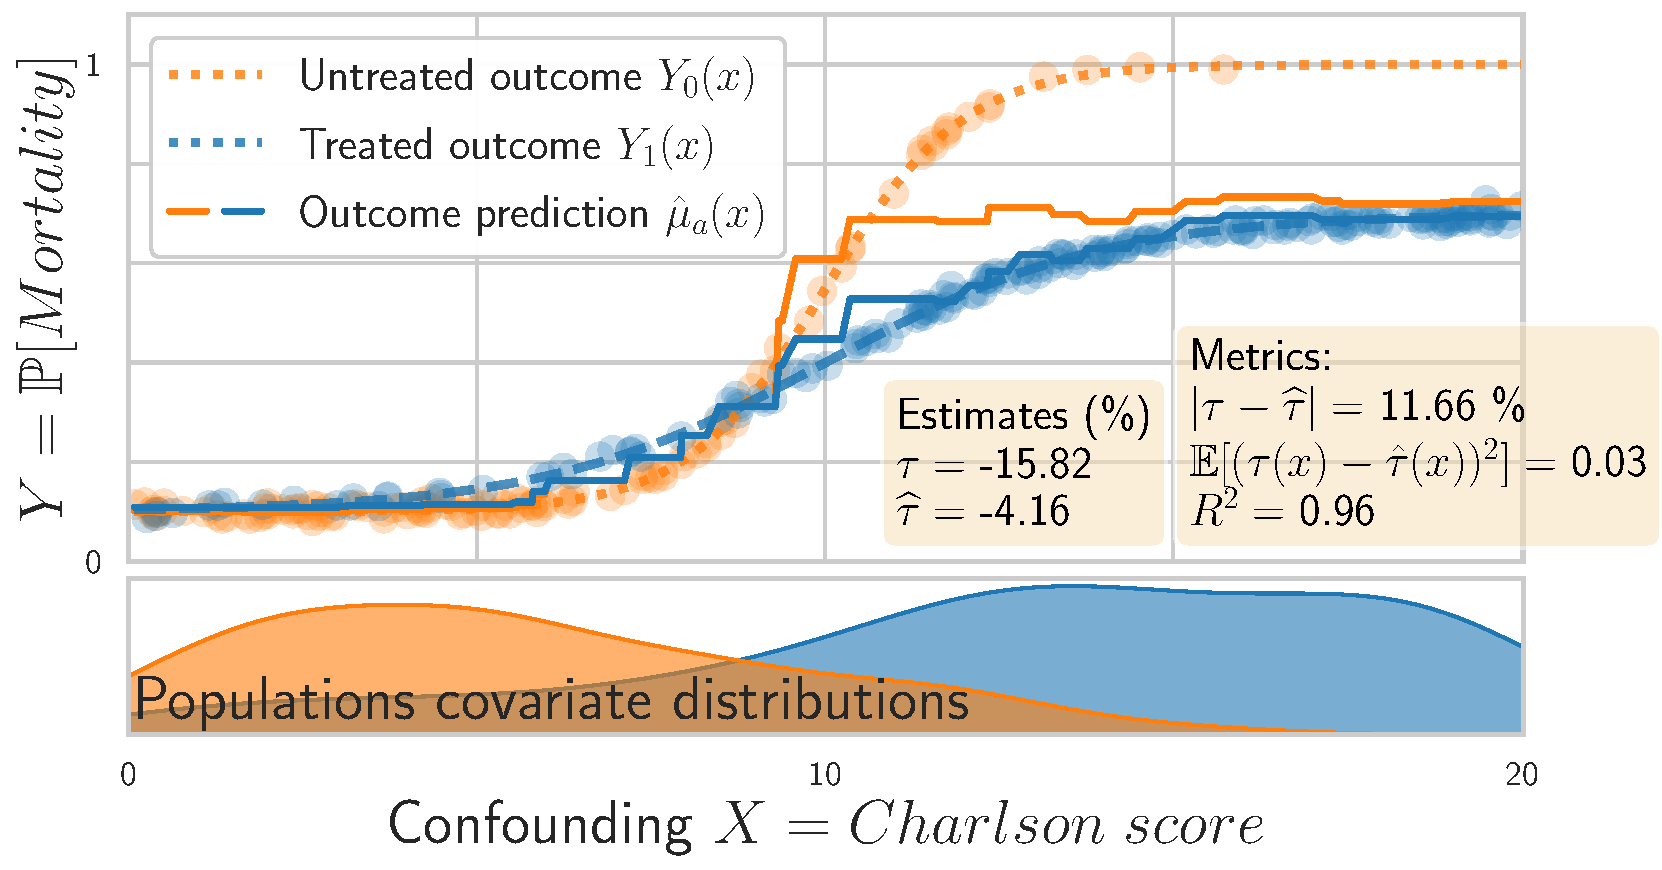
\includegraphics[width=1\linewidth]{toy_random_forest_high_R2_high_tau_risk.pdf}}%
            \put(7.05,4.4){\vector(0,1){.47}}
            \put(7.05,4.4){\vector(0,-1){.55}}
            \put(7.1,4.5){\scriptsize\sffamily treatment effect}
            \put(7.1,4.15){\small $\tau(x)$}
            \put(5.2,3.6){\small $\hat{\tau}(x)$}
            \put(5.15,3.6){\vector(0,1){.29}}
            \put(5.15,3.6){\vector(0,-1){.15}}
        \end{picture}

        {\sffamily\footnotesize\scalebox{0.95}{b) Linear model, worse average
            prediction but better causal inference}}

        \hfill%
        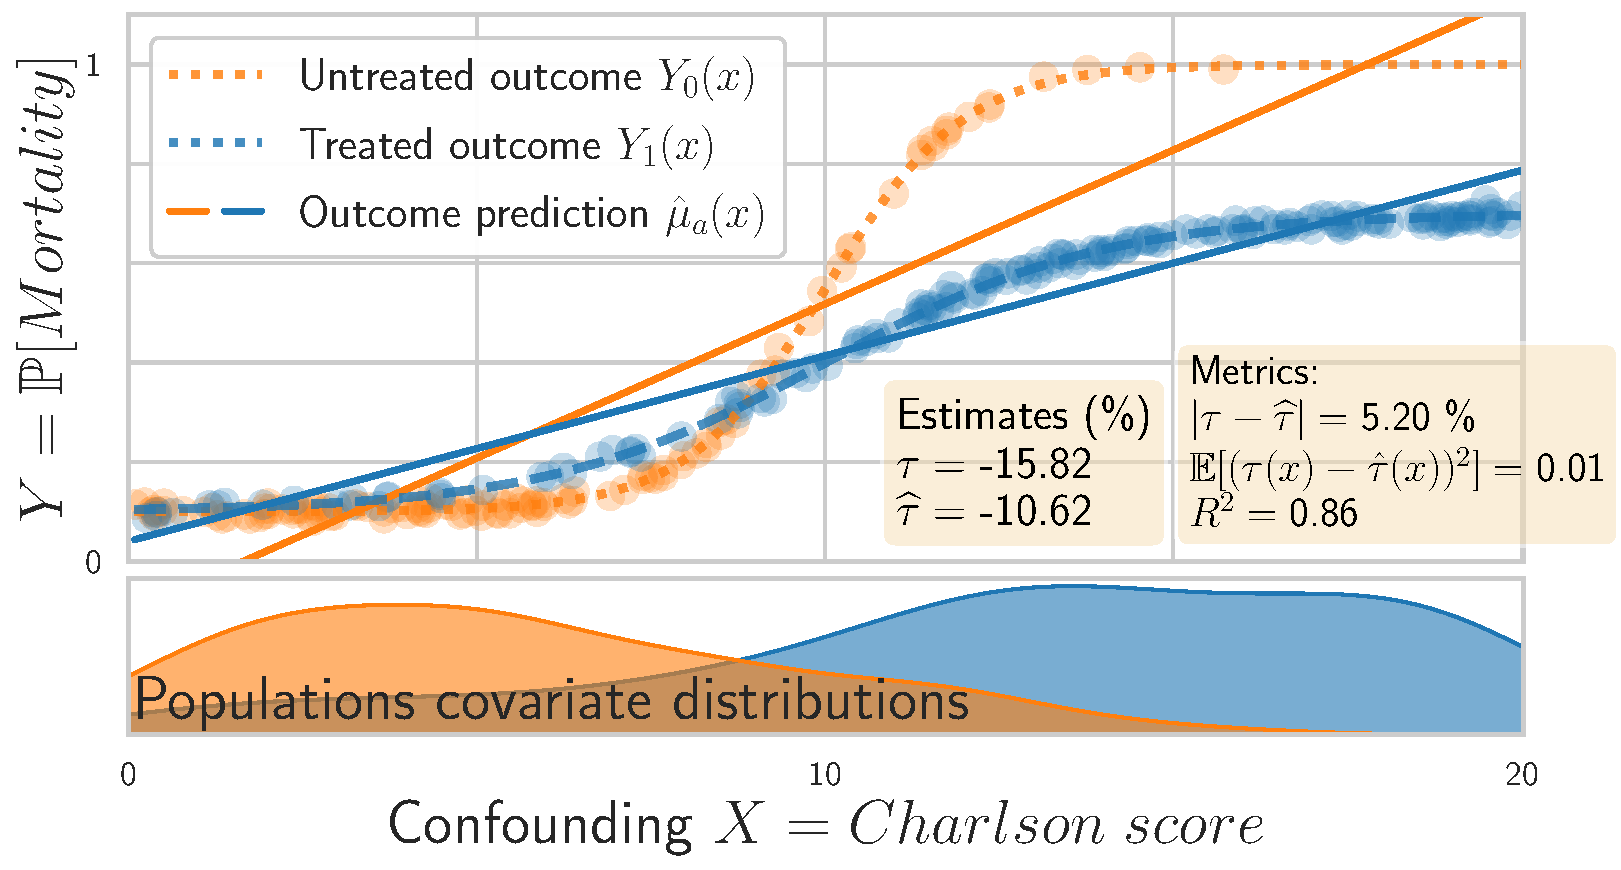
\includegraphics[width=1\linewidth]{toy_tlinear_model_small_R2_small_tau_risk.pdf}%
    \end{minipage}

    \caption[The best predictor may not estimate best causal
        effects]{\textbf{Illustration}: a) a random-forest predictor
        with high performance for standard prediction (high $R^2$) but that
        yields poor causal estimates (large error between true effect $\tau$ and
        estimated $\hat{\tau}$), b) a linear predictor with smaller
        prediction performance leading to better causal estimation. \\[1ex]
        Selecting the predictor with the smallest error to the individual
        treatment effect $\mathbb{E}[(\tau(x) - \hat{\tau}(x))^2]$
        --the $\tau\text{-risk}$, eq.\,\ref{eq:tau_risk} -- would lead to
        the best causal estimates; however computing this error is not
        feasible: it requires access to unknown quantities:
        $\tau(x)$. \\[1ex]
        While the random forest fits the data better than the linear model, it
        gives worse causal inference because its error is inhomogeneous between
        treated and untreated. The $R^2$ score does not capture this
        inhomogeneity.
        \label{fig:toy_example}
    }
\end{figure}


\subsection{Illustration: the best predictor may not estimate best causal
    effects}%

Using a predictor to reason on causal effects relies on contrasting the
prediction of the outcome for a given individual with and without the treatment.
%
Given various predictors of the outcome, which one should we use?
%
Standard predictive modeling or machine-learning practice selects the predictor
that minimizes the expected error on the outcome
\cite{poldrack2020establishment,varoquaux2022evaluating}. However, this
predictor may not be the best model to reason about causal effects of an
intervention as Figure \ref{fig:toy_example} illustrates. Consider the
probability $Y$ of an undesirable outcome (\eg death), a binary treatment $A \in
    \{0, 1\}$, and a covariate $X \in \mathbb R$ summarizing the patient health
status (\eg the Charlson index \cite{charlson_new_1987}). We simulate a
treatment beneficial (decreases mortality) for patients with high Charlson
scores (bad health status) but with little effect for patients in good condition
(low Charlson scores).


Figure \ref{fig:toy_example}a shows a random forest predictor with a
counter-intuitive behavior: it predicts well on average the outcome (as measured
by a regression $R^2$ score) but perform poorly to estimate causal quantities:
the average treatment effect $\tau$ (as visible via the error $|\tau -
    \hat{\tau}|$) or the conditional average treatment effect (the error
$\mathbb{E}[(\tau(x) - \hat{\tau}(x))^2]$, called CATE).
%
On the contrary, Figure \ref{fig:toy_example}b shows a linear model with
smaller $R^2$ score but better causal inference.%

The problem is that causal estimation requires controlling
an error on both treated and non-treated outcome for the same individual:
the observed outcome, and the non-observed \emph{counterfactual} one.
The linear model is misspecified --the outcome functions are not
linear--, leading to poor $R^2$; but it interpolates better to regions
where there are few untreated individuals --high Charlson score-- and
thus gives better causal estimates. Conversely, the random forest puts
weaker assumptions on the data, thus has higher $R^2$ score but is biased
by the treated population in the poor-overlap region, leading
to bad causal estimates.

This toy example illustrates that the classic minimum mean squared error (MSE)
criterion is not suited to choosing a model among candidate
estimators for causal inference.

% A natural way to select a predictive model for causal inference would be

% an error measure between a causal quantity such as the CATE and models' estimate. But such error is
% not a ``feasible'' risk: it cannot be computed solely from observed data
% and requires oracle knowledge.

\section{Methods}\label{sec:framework}
\subsection{Neyman-Rubin Potential Outcomes framework}%
\label{sec:neyman_rubin}%

We first expose the classic construction of the outcome modeling (or
G-computation) estimators of causal effect
\cite{robins_new_1986,snowden_implementation_2011,hernan_causal_2020}.

\paragraph{Settings}

The Neyman-Rubin Potential Outcomes framework
\cite{naimi2023defining,imbens_causal_2015} enables statistical reasoning on
causal treatment effects: Given an outcome $Y \in \mathbb R$ (\eg mortality risk
or hospitalization length), function of a binary treatment $A \in \mathcal{A} =
    \{0, 1\}$ (\eg~a medical procedure), and baseline
covariates $X \in \mathcal{X} \subset \mathbb{R}^d$, we observe the factual
distribution, $O = (Y(A), X, A) \sim \mathcal D = \mathbb P(y, x, a)$. However,
we want to model the existence of potential observations (unobserved ie.~counterfactual) that correspond to a different treatment. Thus we want
quantities on the counterfactual distribution $O^{*} = (Y(1), Y(0), X, A) \sim
    \mathcal D^{*} = \mathbb P(y(1), y(0), x, a)$.

Popular quantities of interest (estimands) are:
at the population level, the
Average Treatment Effect
\begin{flalign*}
    \text{ATE} &  &
    \tau \myeq \; \mathbb{E}_{Y(1),Y(0) \sim \mathcal D^*}[Y(1) - Y(0)];
               &  &
\end{flalign*}
at the individual level, to model heterogeneity, the Conditional Average Treatment Effect
\begin{flalign*}
    \text{CATE} &  &
    \tau (x) \myeq \; \mathbb{E}_{Y(1),Y(0) \sim \mathcal{D}^\star}[Y(1) - Y(0) | X=x].
                &  &
\end{flalign*}

\paragraph{Causal assumptions}

A given data needs to meet a few assumptions to enable identifying
causal estimands \cite{rubin_causal_2005}. \emph{1)} an individual's
outcome $Y$ is solely governed by the corresponding potential outcome:
\begin{flalign}
    \text{\emph{Consistency} assumption,}
     &  &
    Y = A\, Y(1) + (1 - A)\, Y(0)
    \label{eq:consistency}
     &  &
\end{flalign}
\emph{2)}
\emph{unconfoundedness} \mbox{$\{Y(0),
        Y(1) \} \indep A | X$}, \emph{~3)} \emph{strong overlap} ie. every patient has a
strictly positive probability to receive each treatment,
and \emph{4)} \emph{generalization} --no covariate shift.
These classic assumptions, called
\emph{strong ignorability}, are formally detailed in
\ref{apd:causal_assumptions}.

\paragraph{Identifying treatment effects with outcome models -- g-computation \cite{robins_new_1986}}\label{subsec:estimators}

Should we know the two potential outcomes for a given $X$,
we could compute the
difference between them, which gives the causal effect of the treatment.
%
These two potential outcomes can be estimated from observed data:
the consistency and unconfoundedness
\ref{apd:causal_assumptions} assumptions imply the following
equality, linking the target quantity to the observed data:
\begin{equation}\label{eq:mu_identification}
    \mathbb E_{Y(a) \sim \mathcal{D^{\star}}} [Y(a)|X=x] = \mathbb E_{Y \sim \mathcal{D}} [Y|X=x, A=a]
\end{equation}
On the left, the expectation is taken on the counterfactual unobserved
distribution. On the right, the expectation is taken on the factual observed
distribution conditionally on the treatment. For the rest of the
paper, the expectations will always be taken on the factual observed
distribution $\mathcal{D}$. This identification leads to outcome based estimators (ie.
g-computation estimators \cite{snowden_implementation_2011}):
\begin{eqnarray}
    \tau =& \mathbb E_{Y \sim \mathcal{D^{\star}}}[Y(1) - Y(0)]
    \notag
    \\
    = &\mathbb E_{Y \sim \mathcal{D}}[Y|A=1] - \mathbb E_{Y \sim \mathcal{D}}[Y| A=0]
    \label{eq:tau_population}
\end{eqnarray}
This equation builds on the conditional expectation of the outcome given the treatment $\mathbb E_{\sim \mathcal{D}}[Y|A]$. Outcome based methods target this quantity conditionally on the covariates, called \emph{response function}:
\begin{flalign*}
    \text{Response function}
     &  &
    \mu_{a}(x) \myeq \; \mathbb E_{Y \sim \mathcal{D}} [Y|X=x, A=a]
     &  &
\end{flalign*}

Given a sample of data and the oracle response functions $\mu_0, \mu_1$, the
finite sum version of \autoref{eq:tau_population} leads to an unbiased
estimator of the ATE written:
\begin{equation}
    \hat \tau = \frac{1}{n} \biggl(\sum_{i=1}^n \mu_{1}(x_i) - \mu_{0}(x_i) \biggr)
    \label{eq:ate_estimate}
\end{equation}
This estimator is an oracle \emph{finite sum} estimator by opposition to the
population expression of $\tau$, $\mathbb{E}[\mu_{1}(x_i) - \mu_{0}(x_i)]
$,
which involves an expectation taken on the full
distribution $\mathcal D$, which is observable but requires infinite data. For
each estimator $\ell$ taking an expectation over $\mathcal D$, we use the symbol
$\hat \ell$ to note its finite sum version.
The formulas in Eq. (\ref{eq:mu_identification}-\ref{eq:ate_estimate}) are all partly oracle formulas: they rely on
conditional expectations, the response functions, but give no specific
procedures on how to compute or select them. This last point is the topic
of our work, describe in the next section.
%In practice the response function can be estimated with one statistical model taking the treatment as a supplementary covariate $\hat \mu(x, a)$ (called S-learner) or by two separate model fitted on each population, treated or not $(\hat \mu_0(x), \hat \mu_1(x))$ (T-learner) \cite{kunzel_metalearners_2019}.

Similarly to the ATE, at the individual level Eq.\ref{eq:mu_identification} links the CATE to statistical quantities:
\begin{equation}
    \tau(x) = \mu_{1}(x) - \mu_{0}(x)
    \label{eq:cate_estimate}
\end{equation}

\paragraph{Robinson decomposition}
G-computation is a choice of decomposition of the CATE estimation. Other choices
of decomposition exist, such as the R-decomposition
\cite{robinson_rootnconsistent_1988}. The latter introduces two new statistical
estimates, the conditional mean outcome and the probability of being treated (known
as propensity score \cite{rosenbaum_central_1983}):
\begin{flalign}
    \text{Conditional mean outcome} &                    & m(x) \myeq \; & \mathbb E_{Y \sim
    \mathcal{D}} [Y|X=x]            &                    &
    \label{def:m}
    \\
    \text{Propensity score}         &                    &
    e(x) \myeq \;                   & \mathbb P[A=1|X=x]
    \label{def:propensity_score}
\end{flalign}
with these, the outcome (Eq.\,\ref{eq:consistency}) can be written
\begin{flalign}\label{eq:r_decomposition}
    \text{R-decomposition}            &  & y(a) = m(x) + \big( a - e(x) \big)
    \tau(x) + \varepsilon(x; a)\notag &  &
    \\\ &&\text{with}\quad \mathbb E[\varepsilon(X; A)|X, A] = 0&&
\end{flalign}
$m$ and $e$ are often called
\emph{nuisances} \cite{chernozhukov_double_2018}. They are unknown and must be estimated from the data.

\bigskip

Both the in the ATE and CATE formula Eq.\,(\ref{eq:ate_estimate},
\ref{eq:cate_estimate}), and the Robinson decomposition involve
conditional expectations --the response functions $\mu_a(x)$ or the
nuisances $m(x)$ and $e(x)$. In practice those are given by statistical
models: linear models, random forests, etc
\cite{kaddour2022causal,chernozhukov2024applied}.


%As noted by \cite{johansson2022generalization}, the machine learning
%community often referred to the CATE by ITE, the Individual Treatment Effect.
%From a purely causal point of view, the ITE is uniquely defined for each
%individual and might not be accessible: $ITE(x_i) = Y_i(1) -  Y_i(0)$. On the
%contrary, the CATE can always be derived by taking conditional expectancies. It
%is the expected effect of the treatment in the region of the covariate space
%around X. %Too cultivate

\begin{table*}[bt!]
    \makebox[\textwidth]{
        \begin{threeparttable}[b]
            \caption{Review of causal risks
                ---
                The $R\text{-risk}^*$ is called $\tau \text{-risk}_R$ in
                \cite{schuler_comparison_2018}.
                \label{tab:evaluation_metrics}}
            \centering
            \begin{tabular}{llr}
                \toprule
                Risk                                                                                           & Equation
                                                                                                               & Reference                                                                                                                                           \\
                \midrule
                $\tau\text{-risk}=\text{MSE}(\tau(X), \tau_f(X))$                                              & $\mathbb E_{X\sim
                            p(X)}[(\tau(X) - \hat \tau_f(X))^2] $
                                                                                                               & Eq. \ref{eq:tau_risk} \cite{hill_bayesian_2011}                                                                                                     \\
                $\mu\text{-risk} = \text{MSE}(Y, f(X))$                                                        & $\mathbb{E}_{(Y, X, A)
                        \sim \mathcal D}\left[(Y-f(X ; A))^2 \right]$
                                                                                                               & \cite{schuler_comparison_2018}                                                                                                                      \\
                $\mu\text{-risk}_{IPW}^*$                                                                      & $\mathbb{E}_{(Y, X, A)
                        \sim \mathcal D}\left[ \Big( \frac{A}{e(X)} + \frac{1-A}{1-e(X)} \Big)
                (Y-f(X ; A))^2 \right]$                                                                        & \cite{vanderlaan_unified_2003}                                                                                                                      \\
                $\tau\text{-risk}^{\star}_{IPW}$                                                               & $\mathbb{E}_{(Y, X, A) \sim \mathcal D} \left[ \Big(Y \left( \frac{A}{e(X)} - \frac{1-A}{1-e(X)}\right)-\hat \tau_f\left(X\right)\Big)^2 \right]$ &
                \cite{wager_estimation_2018}
                \\
                $U\text{-risk}^*$                                                                              & $\mathbb{E}_{(Y, X, A) \sim \mathcal D}  \big[
                \big( \frac{Y-m\left(X\right)}{A-e\left(X\right)} -  \hat \tau_f\left(X\right)\big)^{2} \big]$ &
                \cite{nie_quasioracle_2017}
                \\
                $R\text{-risk}^*$                                                                              & $\mathbb{E}_{(Y, X, A)
                        \sim \mathcal D} \big[\big(\left(Y-m\left(X\right)\right)
                -\left(A-e\left(X\right)\right) \hat \tau_f\left(X\right)\big)^{2} \big]$                      &
                \cite{nie_quasioracle_2017}
                \\
                \bottomrule
            \end{tabular}
        \end{threeparttable}
    }
\end{table*}


\subsection{Model-selection, oracle and feasible risks}\label{sec:problem:model_selection}


\paragraph{Causal model selection}\label{sec:problem:causal_selection}

We formalize model selection for causal estimation. Thanks to the outcome model identification (\autoref{eq:mu_identification}), a given model $f: \mathcal X
    \times \mathcal A \rightarrow \mathcal{Y}$ --learned from data or built from
domain knowledge-- induces feasible estimates of the ATE and CATE (eqs
\ref{eq:ate_estimate} and \ref{eq:cate_estimate}), $\hat \tau_{f}$ and $\hat \tau_{f}(x)$.
%
However, the g-computation framework presented above is written in terms
of ``perfect'' conditional expectations (oracles), it does not control an
error, \emph{eg} on both populations as highlighted in Figure
\ref{fig:toy_example}. Selection procedures are needed to find the best
conditional-expectation models.

A selection procedure combines a risk $\ell$, evaluating the quality of a
model $f$ with observed data $O$, and a splitting strategy of the data to
estimate different regressions (nuisances) involved in the risk.
%
Formally, let $\mathcal F=\{f: \mathcal X \times \mathcal A \rightarrow \mathcal{Y}\}$ be
a family of such estimators. Our goal is to select the best candidate in this
family for the observed dataset $O$ using a risk
$\ell$:
\begin{equation}
    f^*_{\ell} = \argmin_{f \in \mathcal{F}} \ell(f, O)
    \label{eq:causal_model_selection}
\end{equation}

We now detail possible risks $\ell$, risks useful for causal
model selection, and how to compute them.


\paragraph{The $\tau\text{-risk}$: an oracle error risk}\label{paragraph:oracle_metrics}
%
As we would like to target the CATE, the following
evaluation risk is natural (also called PEHE \cite{schulam_reliable_2017, hill_bayesian_2011}):
\begin{flalign}\label{eq:tau_risk}
    \tau\text{-risk}(f) \myeq \mathbb E_{X\sim p(X)}[(\tau(X) - \hat \tau_f(X))^2]
\end{flalign}

Given observed data from $p(X)$, the expectation is computed with a
finite sum, as in eq.\,\ref{eq:ate_estimate}, to give an estimated
value $\widehat{\tau\text{-risk}}(f)$.
%
However this risk is not feasible as the oracles $\tau(x)$ are
not accessible with the observed data $(Y, X, A) \sim \mathcal D$.

\paragraph{Feasible error risks}\label{paragraph:feasible_metrics} Table
\ref{tab:evaluation_metrics} lists \emph{feasible} risks (Detailed in Appendix
\ref{def:feasible_risks}), based on the prediction error of the outcome model
and \emph{observable} quantities. These observable, called nuisances are $e$
--propensity score, eq \ref{def:propensity_score}-- and $m$ --conditional mean
outcome, eq \ref{def:m}. We give the definitions as \textit{semi-oracles},
function of the true unknown nuisances, but later instantiate them with
estimated nuisances, noted $\big(\check e, \check m \big)$. Semi-oracles risks
are superscripted with the $^{\star}$ symbol.

\subsection{Model selection procedure}\label{problem:estimation_procedure}

Causal model selection (eq
\ref{eq:causal_model_selection}) may involve estimating various quantities
from the observed data: the outcome model $f$, its induced risk as
introduce in the previous section, and possibly nuisances required by the
risk.
Given a dataset with $N$ samples, we split out a train and a test sets
$(\mathcal{T}, \mathcal{S})$. We
fit each candidate estimator $f \in \mathcal{F}$ on $\mathcal{T}$. We also fit
the nuisance models $(\check e, \check m)$ on the train set
$\mathcal{T}$, setting hyperparameters by a nested
cross-validation before fitting the nuisance estimators with these parameters
on the full train set. Causal quantities are then computed by applying the fitted  candidates
estimators $f \in \mathcal{F}$ on the test set $\mathcal{S}$. Finally, we
compute the model-selection metrics for
each candidate model on the test set. This procedure is described in Algorithm
\ref{problem:estimation_procedure:algo} and Figure
\ref{problem:estimation_procedure:figure}.

% As extreme inverse propensity weights induce high variance, clipping can be
% useful for numerical stability
% \cite{swaminathan_counterfactual_2015, ionides_truncated_2008}.

\begin{algorithm}[!htbp]
    \caption{Model selection procedure}\label{problem:estimation_procedure:algo} {%
        Given train and test sets $(\mathcal{T}, \mathcal{S}) \sim \mathcal{D}$,
        a candidate estimator $f$, a causal
        metrics $\ell$:
        \begin{enumerate}
            \item Prefit: Learn estimators for unknown nuisance quantities $(\check e,\,\check m)$ on the training set $\mathcal{T}$
            \item Fit: learn $\hat f(\cdot, a)$ on
                  $\mathcal T$
            \item Model selection: $\forall{x} \in \mathcal{S}$ predict
                  $\big(\hat f(x, 1), \hat f(x, 0)\big)$ and evaluate the estimator storing the metric value: $\ell(f, \mathcal S)$ -- possibly
                  function of $\check e$ and $\check m$
                  %\item Metric evaluation: return the oracle evaluation metrics
                  %evaluated on $\mathcal{S}$: $\big(\widehat{\tau\text{-risk}}(\hat
                  %f^*_{\ell}); \widehat{\ell}_{ATE}(\hat f^*_{\ell}) \big)$
        \end{enumerate}

    }
\end{algorithm}


\begin{figure}[h!]

    \centering\begin{minipage}{.95\linewidth}
        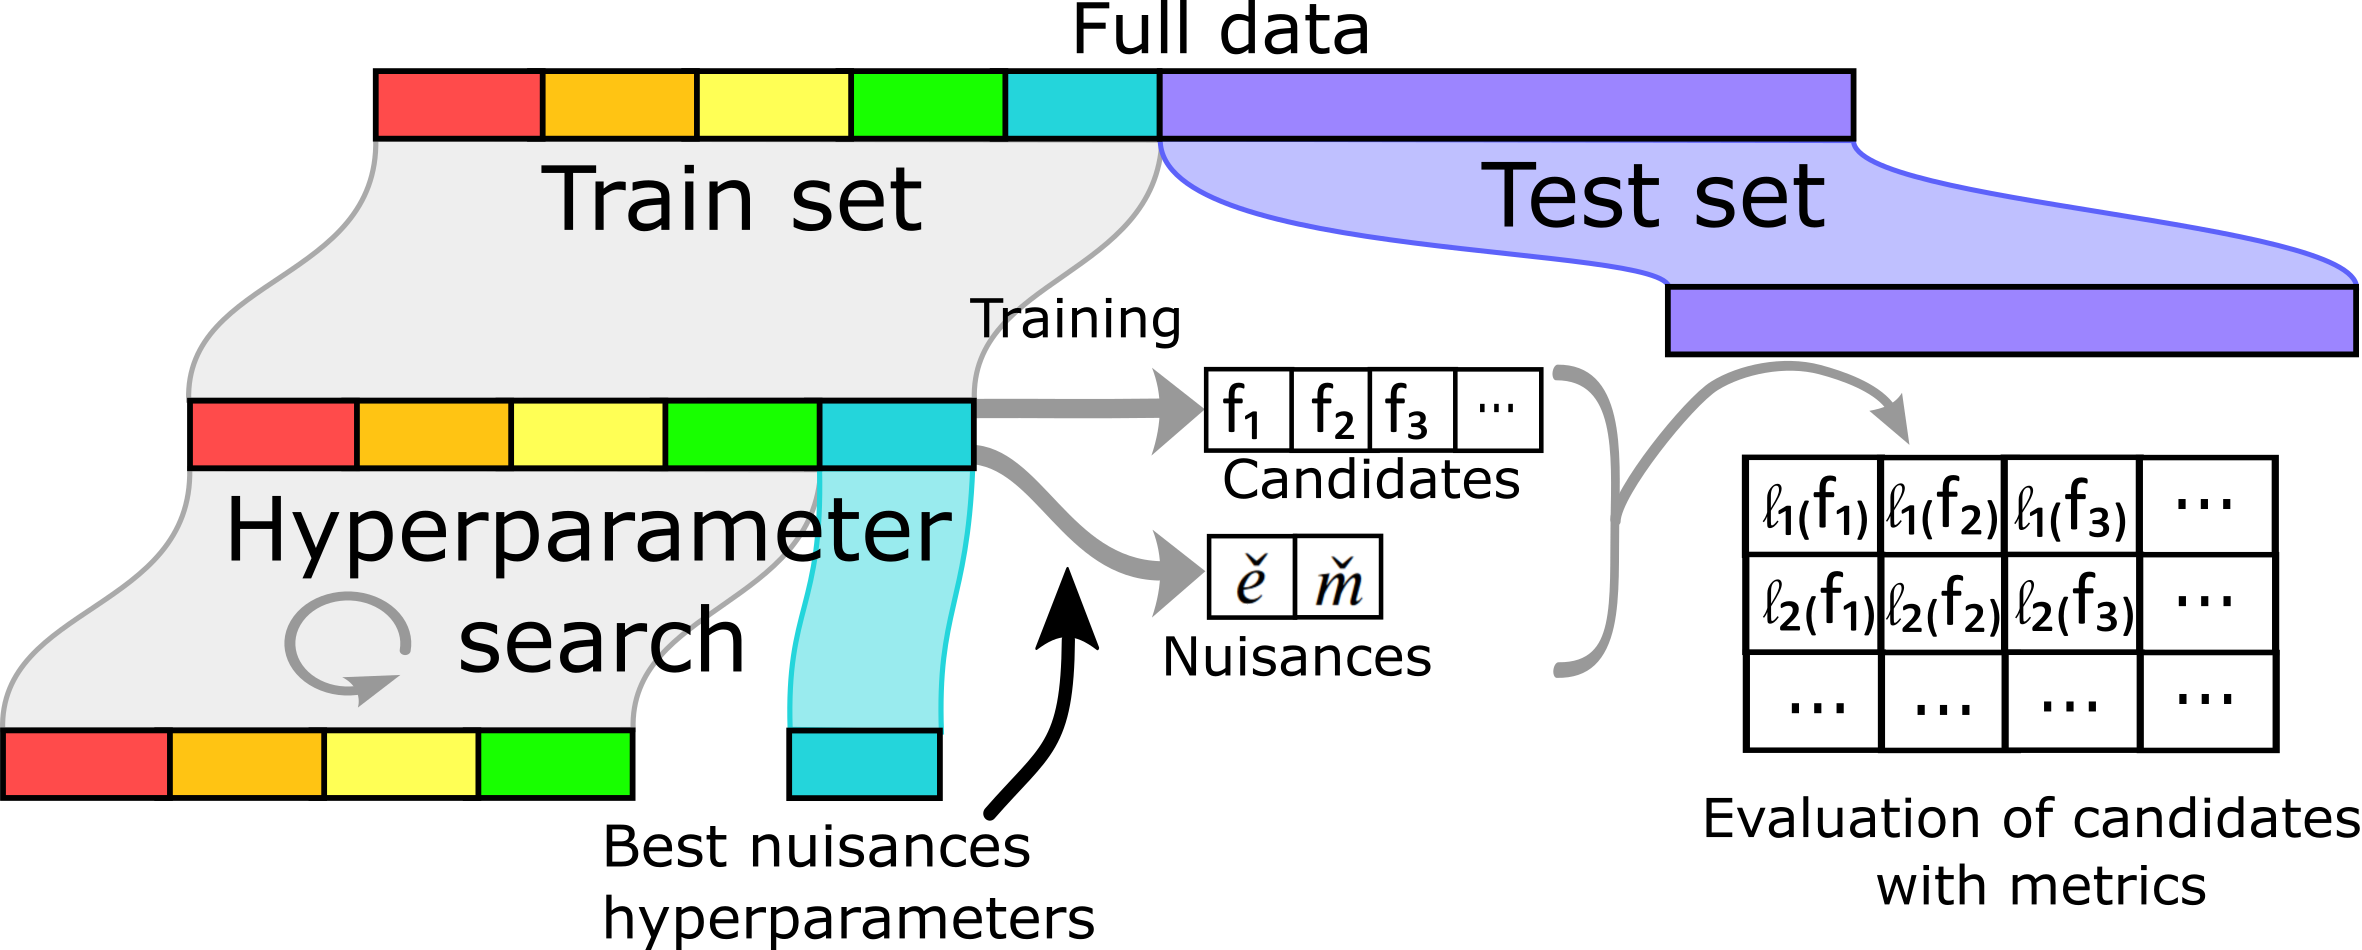
\includegraphics[width=\linewidth]{estimation_procedure_causal_selection_procedure.png}
    \end{minipage}
    \caption{Estimation procedure for causal model
        selection.}\label{problem:estimation_procedure:figure}
\end{figure}



\subsection{R-risk as reweighted oracle metric}\label{theory:r_risk_rewrite}

The $R\text{-risk}$ can be rewritten as a rebalanced $\tau \text{-risk}$.

% We now one feasible risks, $\mu \text{-risk}_{IPW}$ and the
% $R\text{-risk}$ to the oracle $\tau\text{-risk}$. Both results make
% explicit the role of overlap for the performances of causal risks.

This rewriting involves reweighted residuals: for each potential outcome, $a \in
    \{0; 1\}$, the variance conditionally on $x$ is \cite{shalit_estimating_2017}:
\begin{equation*}\label{eq:residuals}
    \sigma_{y}^{2}(x ; a) \overset{\text{def}}{=}
    \int_{y}\left(y-\mu_{a}(x)\right)^{2} p(y \mid x=x ; A=a) \, d y
\end{equation*}
Integrating over the population, we get the Bayes squared error:
$\sigma^2_{B}(a) = \int_{\mathcal X} \sigma_y^2(x;a) p(x)dx$
and its propensity weighted version:
$\tilde{\sigma}^2_{B}(a) = \int_{\mathcal X}\sigma_y^2(x;a)\,  p(x;
    a)\,dx$. In case of a purely deterministic link between the
covariates, the treatment, and the outcome, these residual terms are null.

%\md{Lower bound: I think that there is no lower bound of the tau-risk with the
%mu-risk. That means that we can have a mu risk of 0 wheras the taurisk is
%non-null. Todo for myself: develop an example with overfitted 1NN on the
%observed data.}


\begin{proposition}[$R \text{-risk}$ as reweighted
        $\tau\text{-risk}$]\label{theory:prop:r_risk_rewrite} Given an outcome model
    $f$, its $R\text{-risk}$ appears as weighted version of its $\tau\text{-risk}$
    (Proof in Appendix \ref{apd:proofs}):
    \begin{align}
        R\text{-risk}^*(f) & = \int_{x} e(x)\big(1-e(x)\big)\big(\tau(x)-\tau_ {f}(x)\big)^{2} p(x) d x \nonumber \\
                           & \quad\; + \tilde{\sigma}_B^2(1) + \tilde{\sigma}_B^{2}(0)
    \end{align}
\end{proposition}

The $R \text{-risk}$ targets the oracle at the cost of an overlap re-weighting
and the addition of the reweighted Bayes residuals, which are independent of
$f$. In good overlap regions the weights $e(x) \big(1-e(x) \big)$ are close to
$\frac{1}{4}$, hence the $R \text{-risk}$ is close to the desired gold-standard
$\tau \text{-risk}$. For randomized control trials, this weight is constant
making the $R\text{-risk}$ particularly suited for exploring
heterogeneity (Appendix \ref{apd:proofs})



\section{Empirical Study}\label{sec:empirical_study}

%We now explore empirically the behavior of these different causal selection
%metrics.
%\subsection{Causal metrics under evaluation}

We evaluate the following causal metrics, oracle and feasible
versions, presented in Table
\ref{tab:evaluation_metrics}:\\
$\widehat{\mu\text{-risk}}_{IPW}^*$,
$\widehat{R\text{-risk}}^*$,
$\widehat{U\text{-risk}}^*$,
$\widehat{\tau\text{-risk}_{IPW}}^*$,
$\widehat{\mu\text{-risk}}$,
$\widehat{\mu\text{-risk}}_{IPW}$,
$\widehat{R\text{-risk}}$,
$\widehat{U\text{-risk}}$,
$\widehat{\tau\text{-risk}_{IPW}}$.
We benchmark the metrics in a variety of settings:
many different simulated data generation
processes and three semi-simulated datasets.We provide scripts for the simulations \cite{doutreligne2025caussim} and the selection procedure \cite{doutreligne2025causal}.

The simulations, designed to evaluate the effect of the overlap
parameter, also explore more diverse and noisy covariate distributions.
They cover a diversity of causal settings such as different ratio of causal effect to background responses, and functional links between covariates, outcome and treatment.

\subsection{Caussim: Extensive simulation settings}\label{subsec:simulations}

\paragraph{Data Generation}

We use simulated data, on which the ground-truth causal effect is known. Going
beyond prior empirical studies of causal model selection
\cite{schuler_comparison_2018,alaa_validating_2019}, we use many
generative processes, which is needed to reach general conclusions (Appendix \ref{apd:experiments:additional_results}).

We generate the response functions using random bases extension, a common method
in biostatistics, \eg functional regression with splines
\cite{howe_splines_2011, perperoglou_review_2019}. By allowing the function to
vary at specific knots, we control the complexity of the non-linear outcome
models. We use random approximation of Radial Basis Function (RBF) kernels
\cite{rahimi_random_2008} to generate the outcome and treatment functions. RBF
use the same process as polynomial splines but replace polynomial by Gaussian
kernels. Unlike polynomial, Gaussian kernels have decreasing influences in the
input space. This avoids unrealistic divergences of the functions at the
ends of the feature space. We generate 1\,000 datasets based on these functions,
with random overlap parameters. Example shown in Appendix
\ref{apd:experiments:additional_results}, Fig  13. and details in Appendix \ref{apd:experiments:additional_results}.

\captionsetup[sub]{font=large,labelfont={bf,sf}}%

\paragraph{Family of candidate estimators}

We test model selection across different candidate estimators that
approximate imperfectly the
data-generating process. To build such estimators, we first use an RBF
expansion similar to that used for data generation. We choose two random
knots and transform the raw data features with a Gaussian
kernel. This step is referred as the featurization. Then, we fit a linear
regression on these transformed features. We consider two ways of combining
these steps for outcome model; we use common nomenclature
\cite{kunzel_metalearners_2019,shen2023rctrep} to refer to these different
meta-learners that differ on how they model, jointly or not, the treated and the
non treated:
\begin{itemize}
    \item SLearner: A single learner for both populations, taking the treatment as
          a supplementary covariate.
    \item SftLearner: A single set of basis functions is sampled at random for both
          populations, leading to a given feature space used to model both the treated and
          controls, then two
          separate different regressors are fitted on this shared representation.
    \item TLearner: Two completely different learners for each population, hence
          separate feature representations and regressors.
\end{itemize}

% We do not include more elaborated meta-learners such as R-learner
% \cite{nie_quasioracle_2017} or X-learner
% \cite{kunzel_metalearners_2019}. Our goal is not to have the best possible
% learner but to have a variety of sub-optimal learners to compare the
% different causal metrics. For the same reason, we did not include more powerful
% outcome models such as random forests or boosting trees.

For the regression step, we fit a Ridge regression on the transformed features
with 6 different choices of the regularization parameter $\lambda \in [10^{-3},
        10^{-2}, 10^{-1}, 1, 10^{1}, 10^{2}]$, coupled with a TLearner or
a SftLearner.
We sample 10 different random basis for learning and
featurization yielding a family $\mathcal F$ of 120 candidate estimators.
%

\subsection{Semi-simulated datasets}

\paragraph{Datasets}\label{semi_simulated:datasets}

We also use three semi-simulated
data adding a known synthetic causal effect to real --non synthetic-- healthcare
covariate. ACIC 2016 \cite{dorie_automated_2019} is based on the Collaborative
Perinatal Project \cite{niswander_women_1972}, a RCT studying infants’
developmental disorders containing 4,802 indivduals and 55 features. We used 770
dataset instances: 10 random seeds for each of the 77 simulated settings for the
treatment and outcomes.  ACIC 2018 \cite{shimoni_benchmarking_2018} simulated
treatment and outcomes for the Linked Births and Infant Deaths Database (LBIDD)
\cite{macdorman_infant_1998} with $D=177$ covariates. We used all 432 datasets
of size $N=5\,000$.  Twins \cite{louizos_causal_2017} is an augmentation of real
data on twin births and mortality rates \cite{almond_costs_2005}. There are
$N=11\,984$ samples, and $D=50$ covariates for which we simulated 1,000
different treatment allocations. Appendix
\ref{apd:experiments:additional_results} gives datasets details.


\paragraph{Family of candidate
    estimators}\label{semi_simulated:candidate_estimators}

For these three datasets, the family of candidate estimators are gradient
boosting trees for both the response surfaces and the treatment
(scikit-learn HistGradientBoostingRegressor HistGradientBoostingClassifier  \cite{pedregosa_scikitlearn_2011})
with S-learner, learning rate
in $\{0.01, 0.1, 1\}$, and maximum number of leaf nodes in $\{25, 27, 30, 32,
    35, 40\}$ resulting in a family of size 18.

\paragraph{Nuisance estimators}

Drawing from the TMLE literature that uses combination of flexible
machine learning methods \cite{schuler_targeted_2017}, we model the nuisances
$\check e$ (respectivley $\check m$) with a meta-learner: a stacked estimator of ridge
and boosting classifiers (respectively regressions) (hyperparameter selection in Appendix \ref{apd:experiments:additional_results}).


\subsection{Measuring overlap between treated and non treated}\label{subsec:measuring_overlap}

%\idea{Overlap is important but not easily measurable}
Good overlap between treated and control population is crucial for causal
inference (Assumption \ref{apd:causal_assumptions}). We introduce the
Normalized Total Variation (NTV), a divergence based on the propensity score
summarizing the overlap between both populations (Appendix
\ref{apd:motivation_ntv}).

\begin{figure}[!b]
    % XXX: for submission
    \centering\begin{minipage}{\linewidth}
        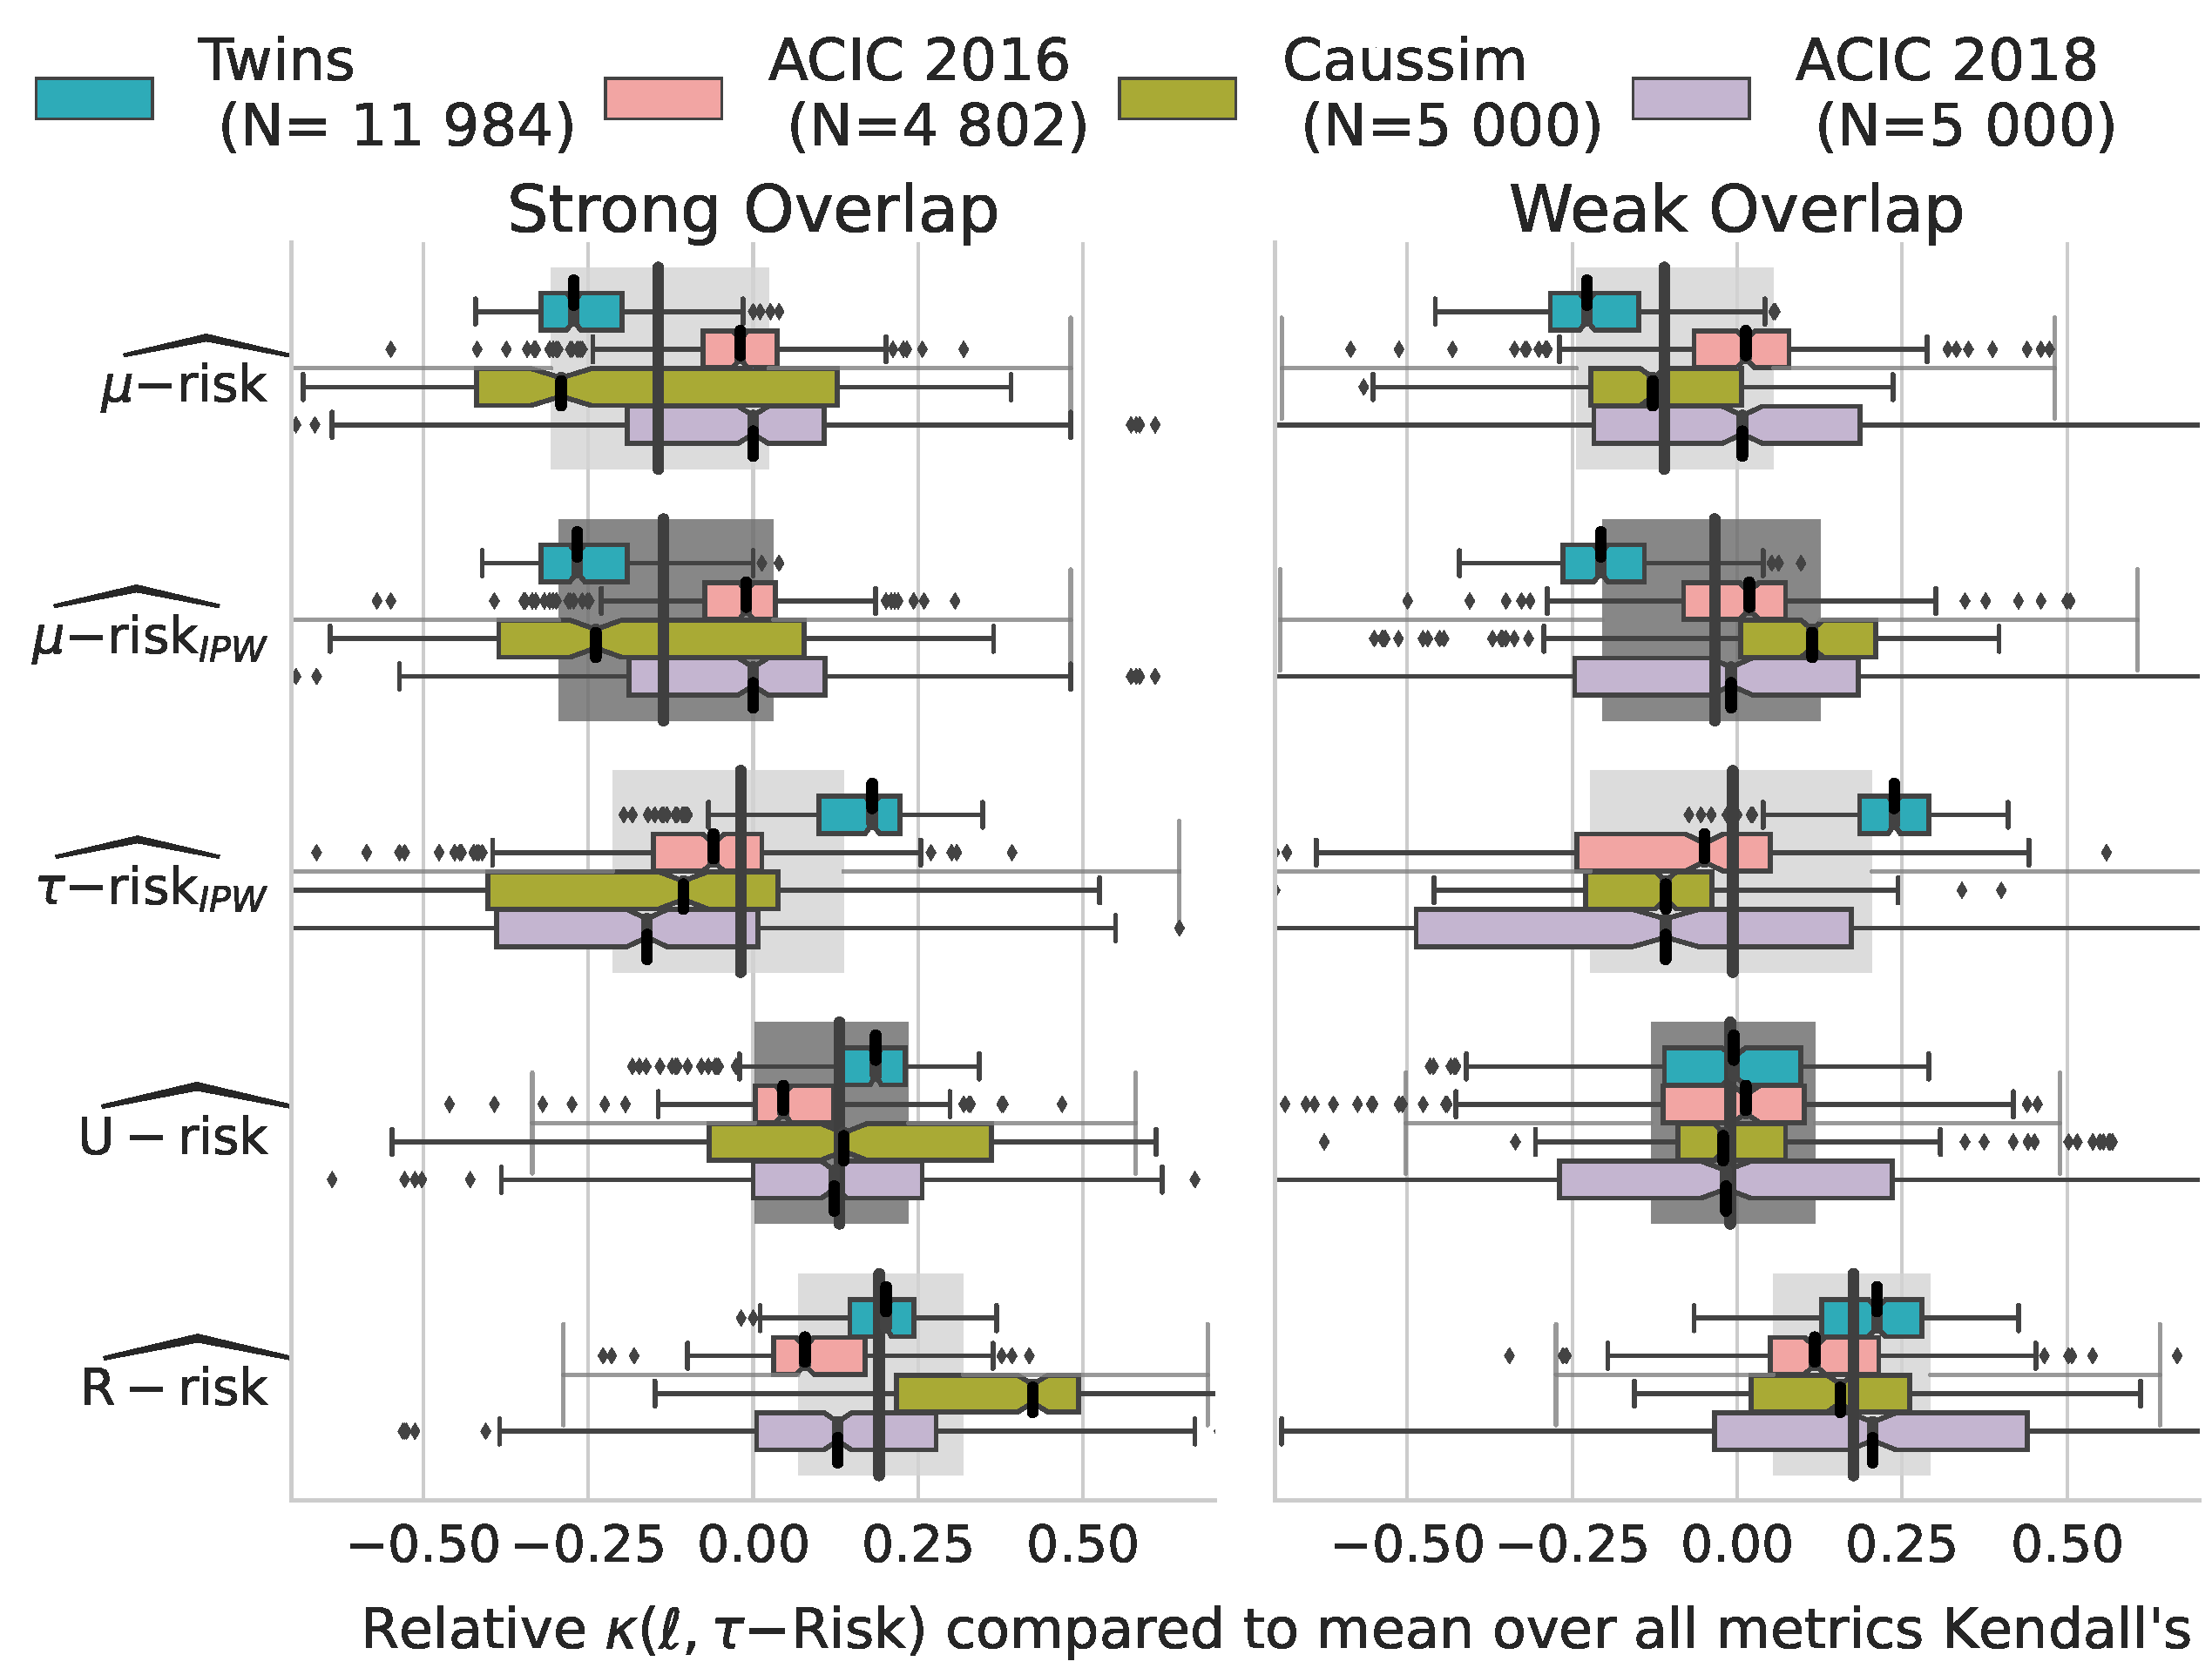
\includegraphics[width=\linewidth]{_1_r_risk_domination_mrisks_by_ds_feasible.pdf}
    \end{minipage}
    \caption{\textbf{The $R$-risk is the best metric}: Relative Kendall's $\tau$ agreement with $\tau\text{-risk}$.
        Strong and Weak overlap correspond to the first and last tertiles of the overlap distribution measured with
        Normalized Total Variation (Appendix \ref{apd:motivation_ntv}). Appendix \ref{apd:experiments:additional_results} presents the same results
        by adding semi-oracle risks in Figure 14, measured with
        absolute Kendall's in Figure 15 and with $\tau\mathrm{-risk}$
        gains in Figure 16. Table
        4 gives median and
        IQR of the relative Kendall.}\label{fig:relative_kendalls_all_datasets}
\end{figure}



\section{Results: factors driving good model selection}\label{empirical_study:results}


\paragraph{The $R\text{-risk}$ is the best metric on average}

Figure \ref{fig:relative_kendalls_all_datasets} shows the agreement between the
ideal ranking of outcome models given the oracle $\tau\text{-risk}$ and the
different feasible causal metrics. We measure this agreement with relative
Kendall tau $\kappa$ (see Appendix \ref{apd:experiments:additional_results}, eq. 20) \cite{kendall_new_1938}. To
remove the variance across datasets (some datasets lead to easier model
selection than others), we report values for one metric relative to the mean of
all metrics for a given dataset instance: $\text{Relative} \,
    \kappa(\ell,\tau\mathrm{{-risk}})= \kappa(\ell,\tau\mathrm{{-risk}}) -
    mean_{\ell}\big(\kappa(\ell,\tau\mathrm{{-risk}})\big)$. Given the importance of
overlap in how well metrics approximate the oracle $\tau\text{-risk}$, we
separate strong and weak overlap.

Among all metrics, the classical mean squared error (ie. factual
$\mu\text{-risk}$) is worse and reweighting it with propensity score
($\mu\text{-risk}_{IPW}$) does not bring much improvements. The
$R\text{-risk}$, which includes a model of mean outcome and propensity
scores, leads to the best performances. Interestingly, the
$U\text{-risk}$, which uses the same nuisances, deteriorates in weak overlap, probably due to variance
inflation when dividing by extreme propensity scores.

Beyond rankings, the differences in terms of absolute
ability to select the best model are large: The R-risk selects a model
with a $\tau\text{-risk}$ only 1\% higher
than the best
possible candidate for strong overlap on Caussim, but selecting with
the $\mu\text{-risk}$ or $\mu\text{-risk}_{IPW}$ --as per machine-learning
practice-- leads to 10\% excess risk and using $\tau\text{-risk}_{IPW}$
--as in some causal-inference methods \cite{athey2016recursive,gutierrez_causal_2016}--leads to 100\% excess risk
(Appendix \ref{apd:experiments:additional_results}, Figure 16). Across
datasets, the $R\text{-risk}$ consistently decreases the
risk compared to the $\mu\text{-risk}$: from
0.1\% to 1\% on ACIC2016,  1\% from to 20\% on ACIC2018,
and 0.05\% from to 1\% on Twins.


\paragraph{Model selection is harder for low population
    overlap}

Model selection for causal inference becomes more and more difficult with
increasingly different treated and control populations (Figure
\ref{fig:all_datasets_overlap_effect_r_risk}). The absolute Kendall's
coefficient correlation with $\tau\text{-risk}$ drops from 0.9
(excellent agreement with oracle selection) to 0.6 on both Caussim and ACIC 2018
(Appendix \ref{apd:experiments:additional_results}, Figure 15).

\begin{figure}[!h]
    % XXX: for submission
    \centering\begin{minipage}{\linewidth}
        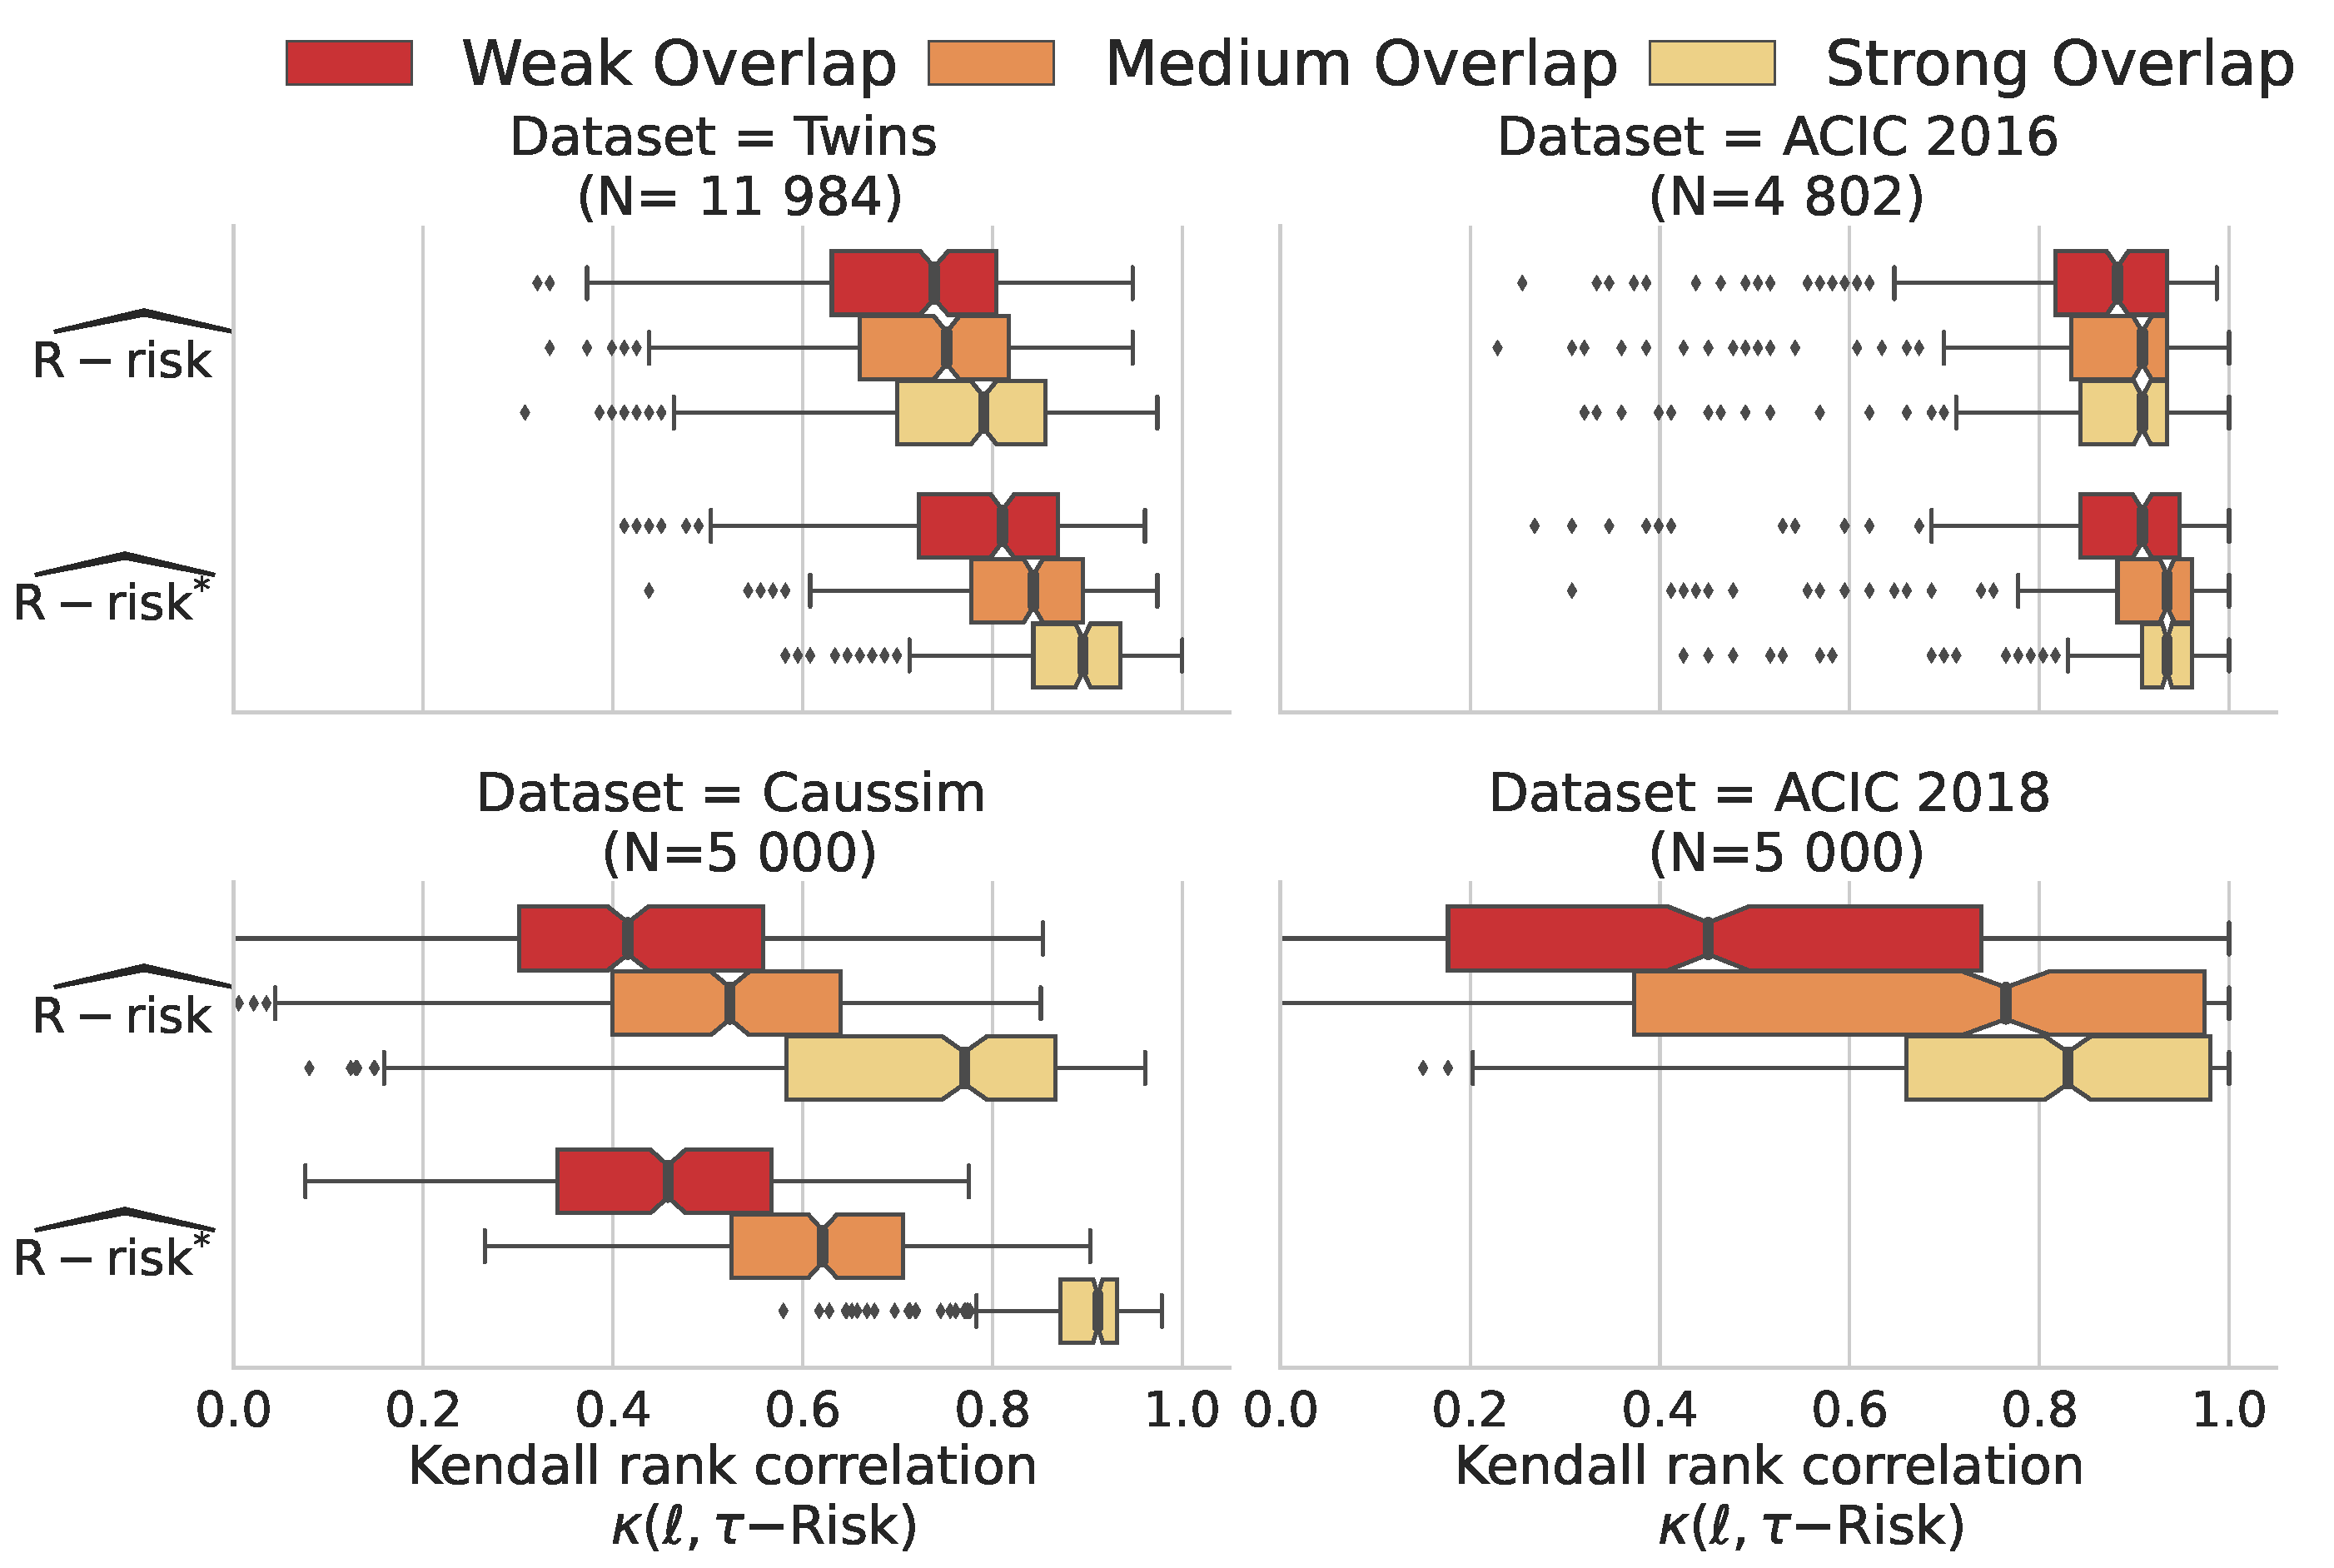
\includegraphics[width=\linewidth]{_2_overlap_influence_by_bin_k_by_ds_r_risk_2cols.pdf}
    \end{minipage}
    \caption{\textbf{Model selection is harder for low population
            overlap}:
        Kendall's $\tau$ agreement with $\tau\text{-risk}$. Strong, medium and Weak overlap
        are the tertiles of the overlap measured with NTV (Appendix \ref{apd:motivation_ntv}, eq. 17). Appendix \ref{apd:experiments:additional_results} presents results for all
        metrics in Figure 18 in absolute
        Kendall's and continuous overlap values in Figure
            {15}.}\label{fig:all_datasets_overlap_effect_r_risk}
\end{figure}



\paragraph{Nuisances can be estimated on the same data as outcome models}

Using the train set $\mathcal{T}$ both to fit the candidate estimator and the
nuisance estimates is a form of double dipping which can lead errors in
nuisances correlated to that of outcome models
\cite{nie_quasioracle_2017}. In theory, these correlations can bias model
selection and, strictly speaking, push
to split out a third separated dataset --a ``nuisance set''-- to fit the
nuisance models. The drawback is that it depletes the data available for
model estimation and selection. However, Figure
\ref{fig:procedures_comparison} shows no substantial difference between a procedure with a separated
nuisance set and the simpler shared nuisance-candidate set procedure.

Empirically, the best split is 90\,\%/10\,\%:
using 90\,\% of the data
to estimate both the nuisances and candidates, then computing the risks on the
remaining test set for model selection (experiments in Appendix
\ref{apd:results:data_split}).

\begin{figure}[!tb]
    % XXX: for submission
    \centering\begin{minipage}{\linewidth}
        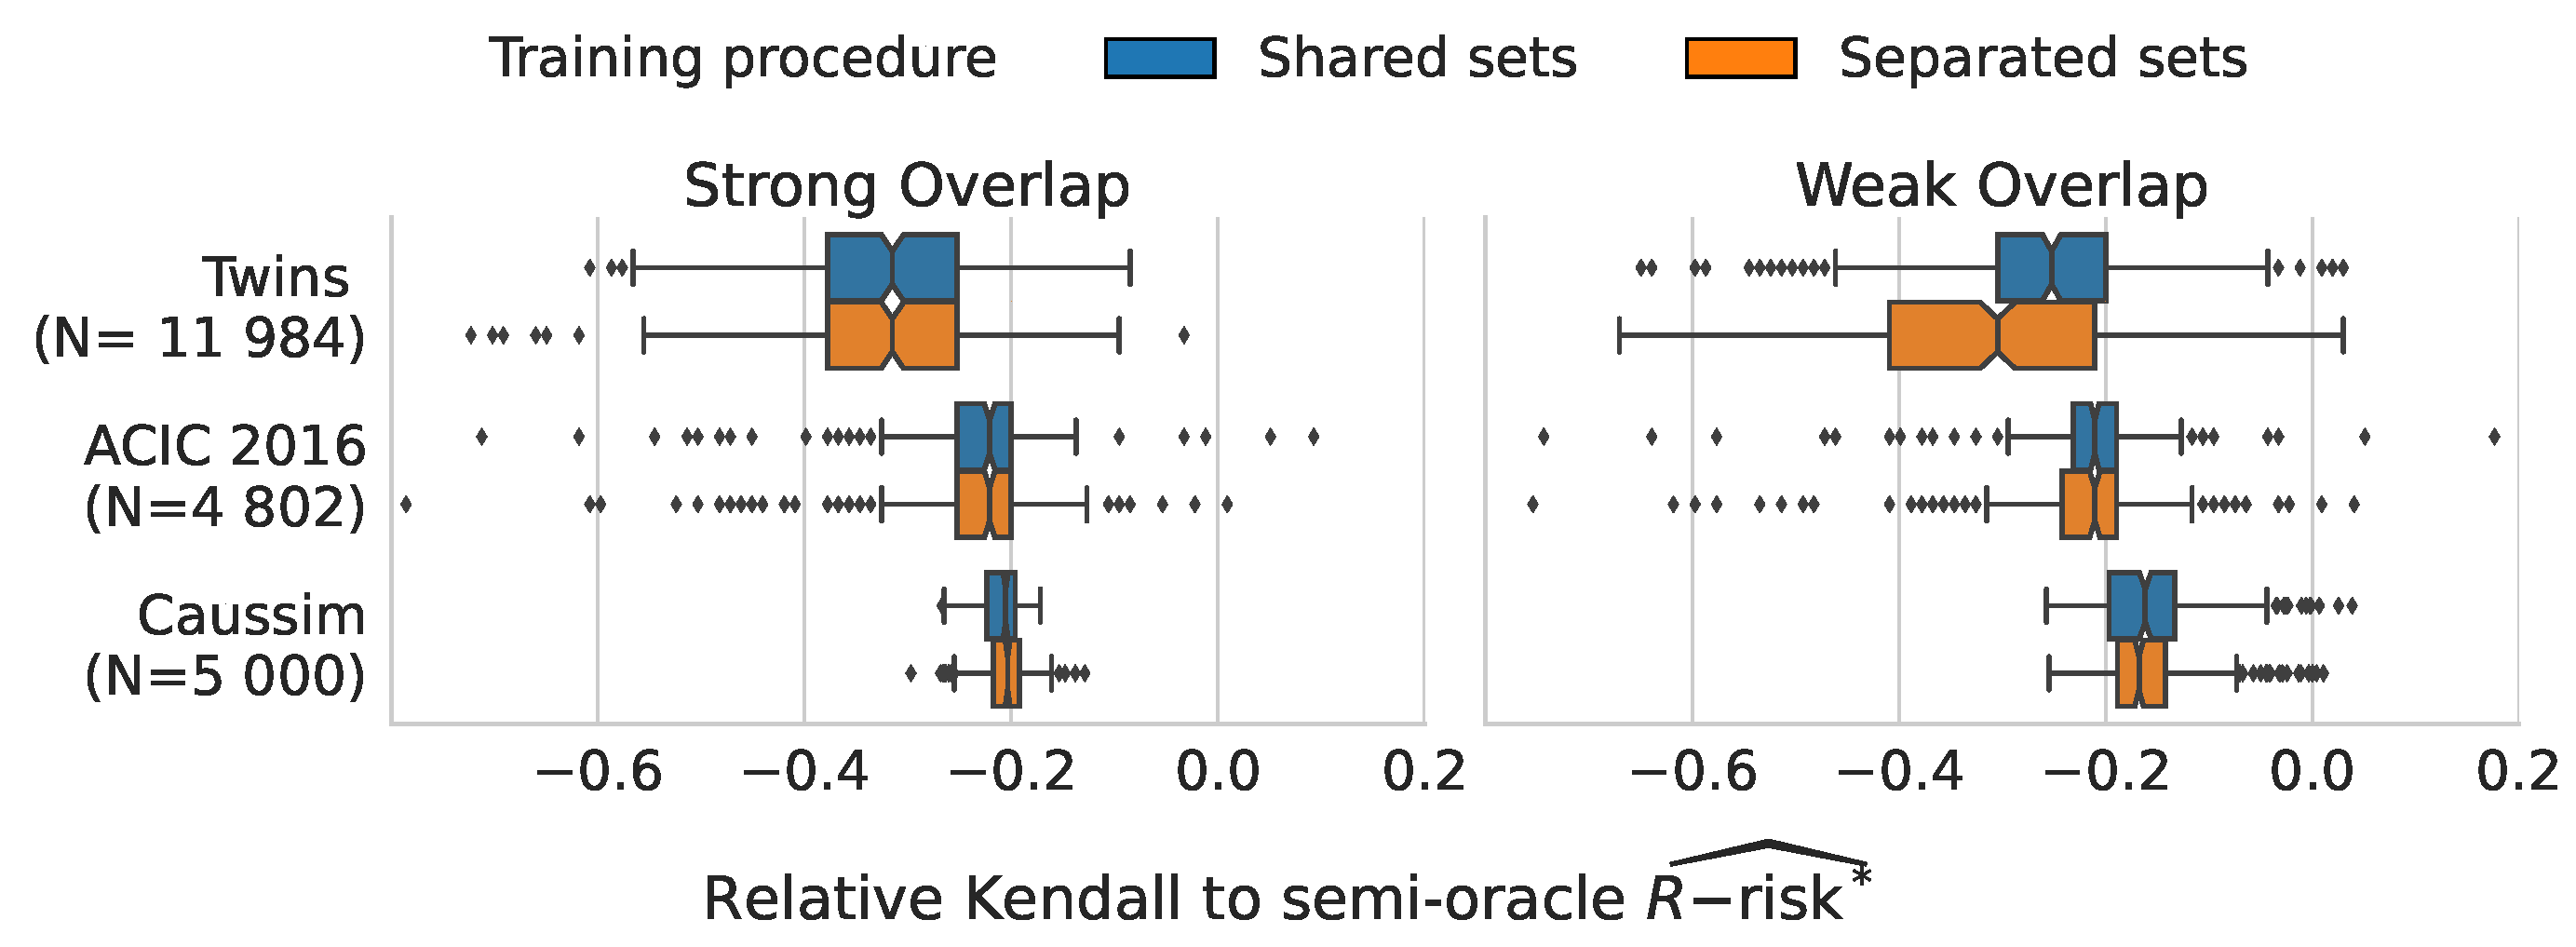
\includegraphics[width=\linewidth]{_3_procedure_r_risk_only_3datasets_twocols.pdf}
    \end{minipage}

    \caption{\textbf{Nuisances can be estimated on the same data as outcome
            models}: Results for the R-risk are similar between the
        \textcolor{MidnightBlue}{shared
            nuisances/candidate set} and
        the \textcolor{RedOrange}{separated nuisances set} procedures. Appendix \ref{apd:experiments:additional_results} Figure
        17 details results for all metrics.}\label{fig:procedures_comparison}
\end{figure}

\paragraph{Stacked models are good overall estimators of nuisances}

Stacked nuisances estimators (boosting and linear) lead to feasible
metrics with close performances to the oracles ones: the
corresponding estimators recover well-enough the true nuisances.
One may wonder if simpler models for the nuisance could be useful,
in particular in data-poor settings or when the true models are linear.
Figure \ref{fig:all_datasets_nuisances_comparison} compares causal model
selection estimating nuisances with stacked estimators or linear model.
It comprises the Twins data, where the true propensity model is linear,
and a downsampled version of this data, to study a situation favorable to
linear models. In these settings,
stacked and linear estimations of the nuisances performs equivalently.
Detailed analysis (Appendix \ref{apd:experiments:additional_results} Figure 20)
confirms that using adaptive models --as built by
stacking linear models and gradient-boosted trees-- suffices to estimate nuisance.

\begin{figure}[!tb]
    % XXX: for submission
    \centering\begin{minipage}{\linewidth}
        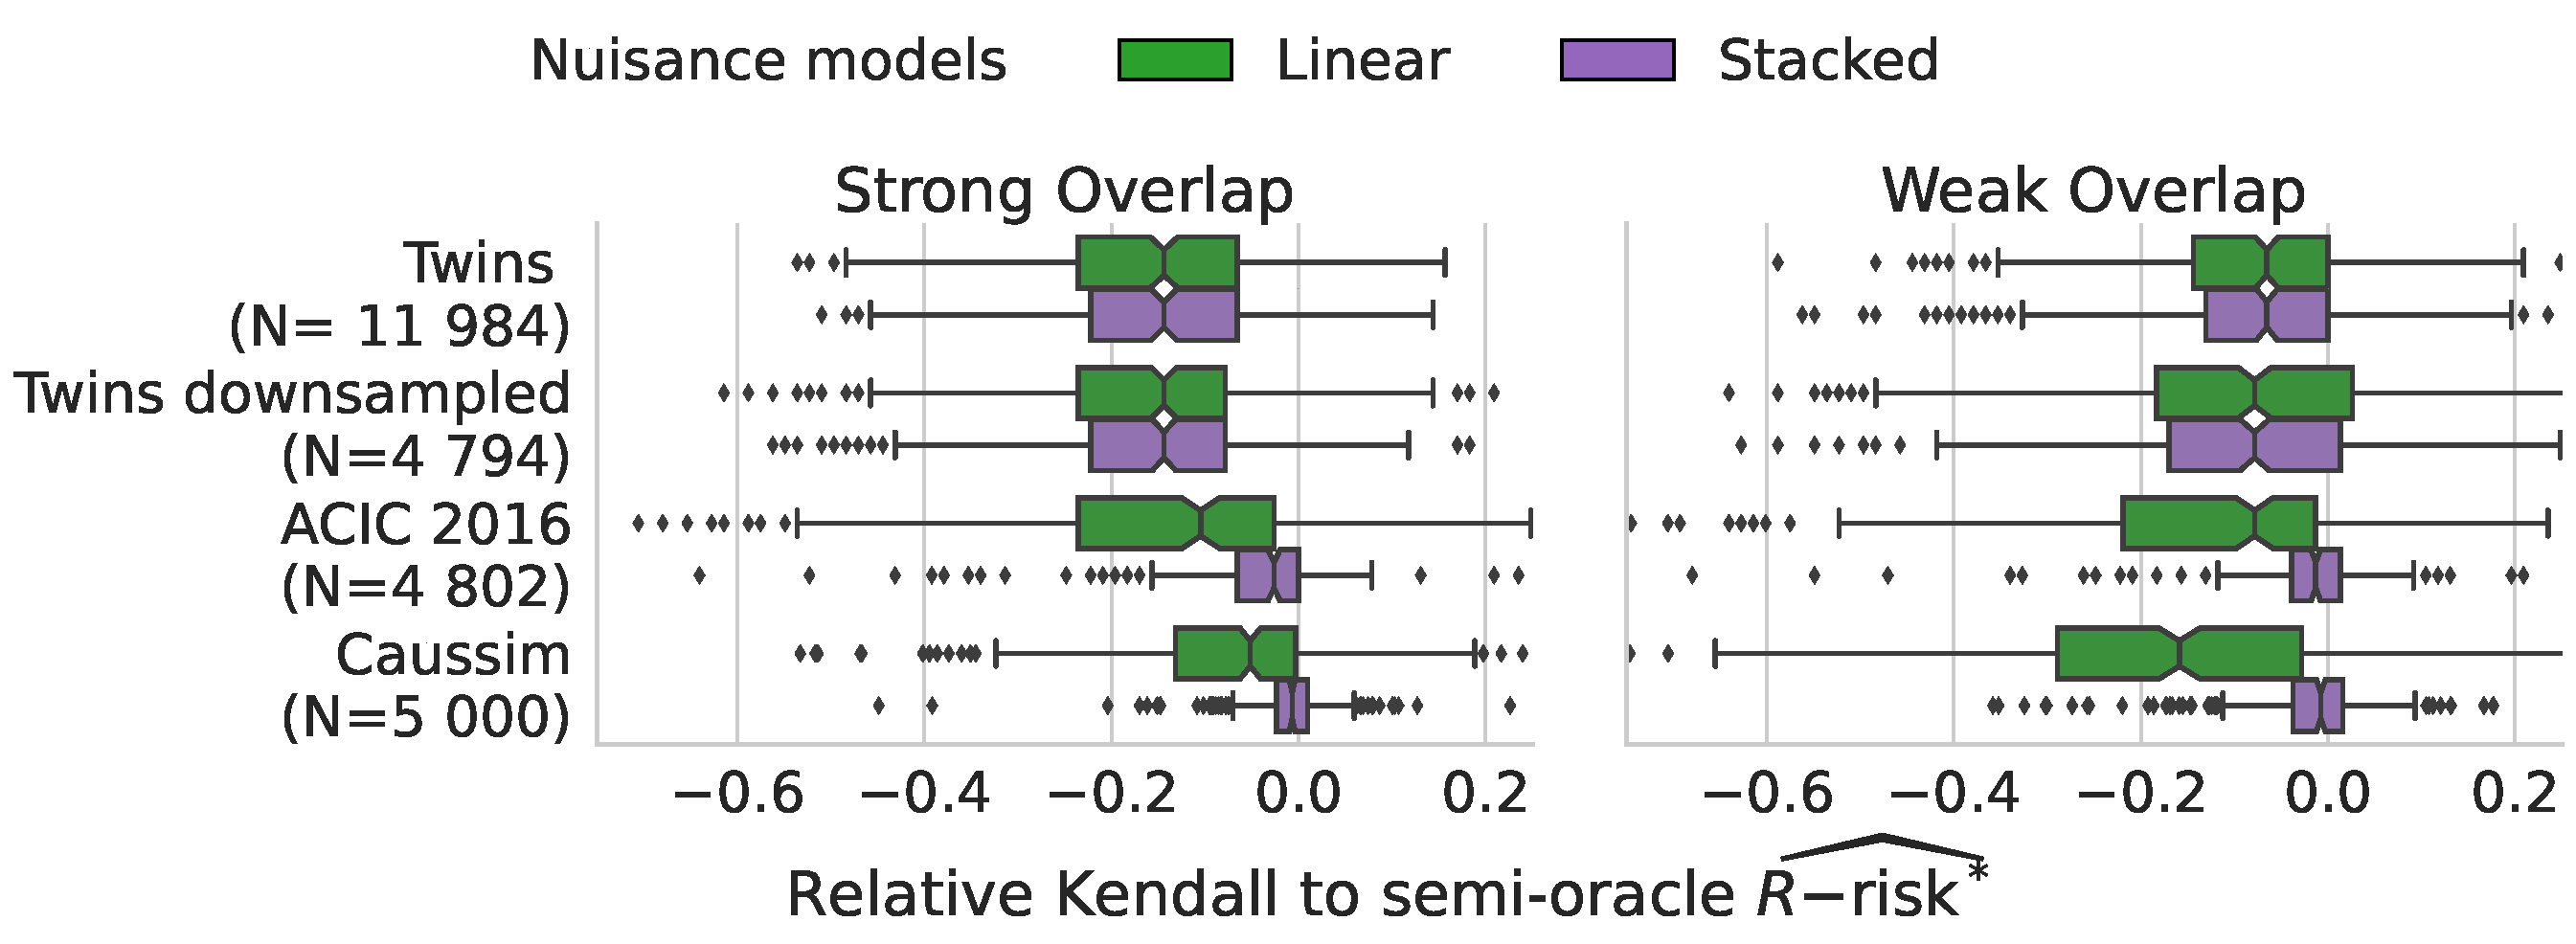
\includegraphics[width=\linewidth]{_4_nuisance_models_r_risk_3ds_2cols.pdf}
    \end{minipage}

    \caption{\textbf{\textcolor{DarkOrchid}{Stacked
                models} are good overall estimators of the nuisances}:
        Results are shown only for the
        R-risk; \ref{apd:experiments:additional_results} Figure 19
        details every metrics. For Twins, where the true propensity
        model is linear, \textcolor{DarkOrchid}{stacked} and
        \textcolor{ForestGreen}{linear}
        estimations of the nuisances performs equivalently, even for a downsampled version
        (N=4,794). }\label{fig:all_datasets_nuisances_comparison}
\end{figure}


\paragraph{R-risk is robust to a wide range of effect ratio values}

Beyond overlap, we study for caussim simulations, the effect on model selection
of different causal effect ratio to baseline. We vary the empirical mean
absolute difference between the causal effect and the baseline, $\Delta_{\mu} = \frac{1}{N} \sum_{i=1}^N \big | \frac{\mu_{1}(x_i) - \mu_{0}(x_i)}{\mu_{0}(x_i) + \mu_{1}(x_i) - \frac{1}{N} \sum_{j=1}^N \mu_0(x_j) + \mu_1(x_j)} \big |$, covering a ratio range from 0.04 to 206 ($\text{median}=9.1$). Appendix \ref{apd:effect_ratio} details this setup as well as an alternive measure of effect ratio. Figure
\ref{fig:effect_ratio_influence} shows that for high values of the ratio,
$R-\text{risk}$ is outperformed by the $\mu\text{-risk}_{IPW}$ and the
$\tau\text{-risk}_{IPW}$. However, on average, the $R-\text{risk}$ is still the
better risk.

\begin{figure}[!tb]
    \centering
    \begin{minipage}{\linewidth}
        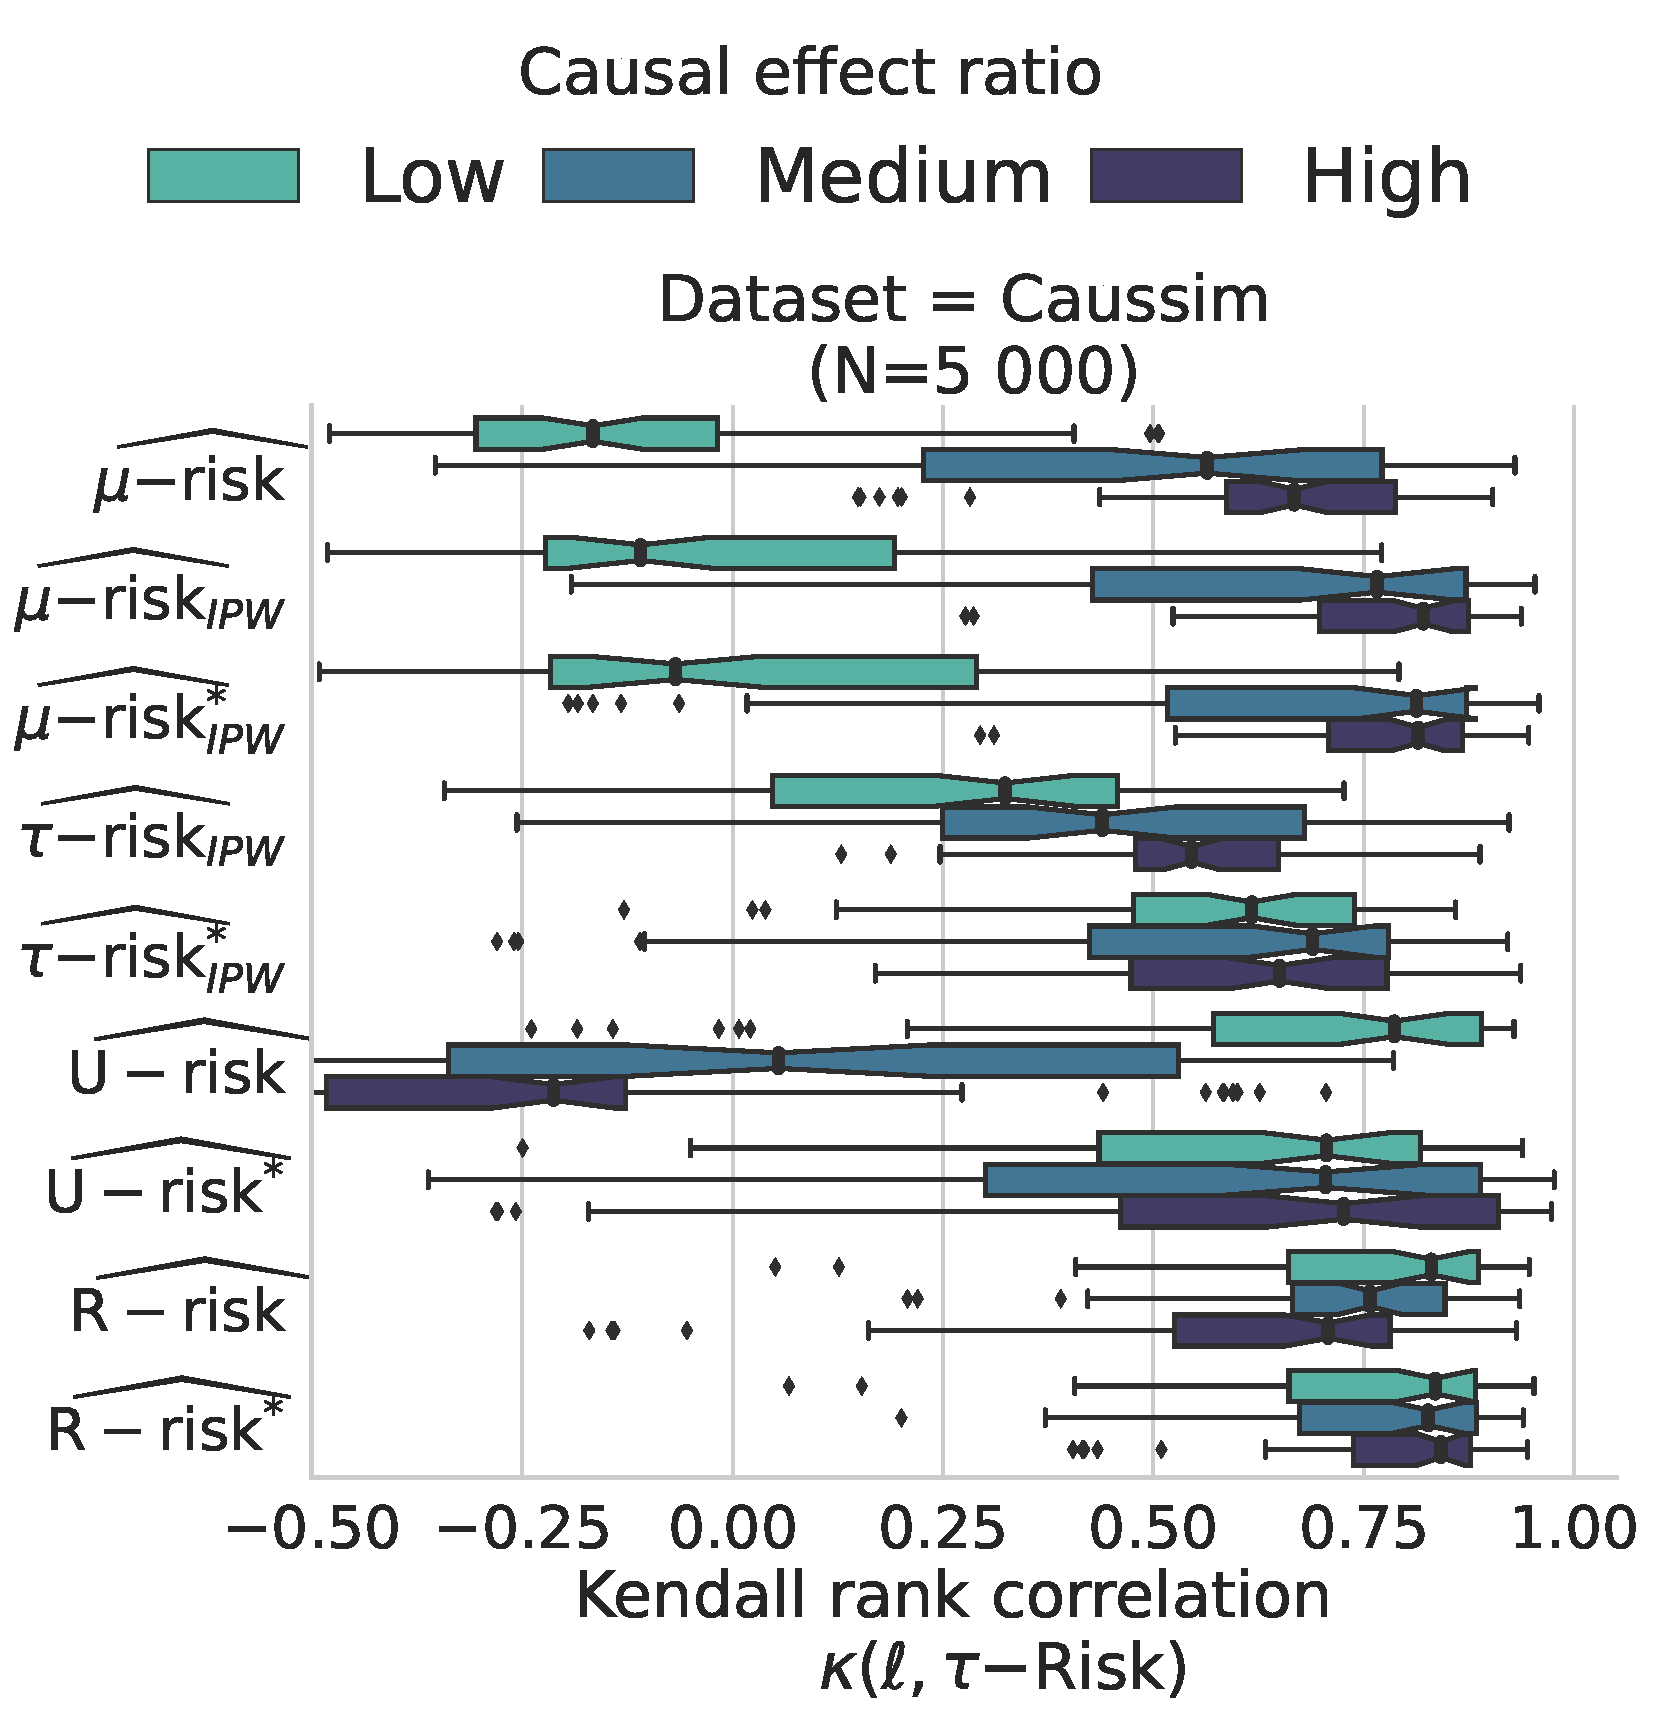
\includegraphics[width=0.9\linewidth]{_6_effect_ratio_sym_by_bin_comparaison_kendall_by_Dataset.pdf}
    \end{minipage}

    \caption{\textbf{R-risk is robust to a wide range of effect ratio}:
    Kendall's $\tau$ agreement with $\tau$-risk. Strong, medium and Weak Causal
    effect ratio are the tertiles of the absolute ratio causal effect to
    baseline response, $\Delta_{\mu}$: Low $[0.04;2.86[$, Medium $[2.86; 16.65[$,
    High $[16.65;206.53[$. Appendix \ref{apd:effect_ratio} details this
    simulation.}\label{fig:effect_ratio_influence}
\end{figure}


\section{Discussion and conclusion}\label{sec:discussion}\label{sec:conclusion}


\paragraph{Nuisance models: more gain than pain}
%
Predictive models are increasingly used to reason about treatment effects, for
instance in precision medicine to drive individualized decision. Our results
highlight that they should be selected, validated, and tuned using different
procedures and error measures than those classically used to assess prediction. Rather, selecting the best outcome
model according to the $R\text{-risk}$ (Appendix \ref{def:feasible_risks} eq.\, Definition 5) leads
to more valid causal estimates on average. Estimating the $R\text{-risk}$ requires a more
complex procedure than standard cross-validation used \eg in machine
learning: it involves fitting nuisance models necessary for model
evaluation.
Our results show that these can be learned on the same set of data as the
outcome models evaluated. The nuisance models must be well estimated (Figure
\ref{fig:all_datasets_nuisances_comparison}). Our results show that using for
nuisance models a flexible stacking-based family of estimator suffices for good
model selection. To select propensity score models, we used the Brier score,
minimized by the true individual probability. An easy mistake is to
use calibration errors popular in machine learning
\cite{platt_probabilistic_1999,zadrozny_obtaining_2001,niculescu-mizil_predicting_2005,minderer_revisiting_2021}
as these select not for the individual posterior probability but for an
aggregate error rate \cite{perez2022beyond}.

%
% However these models are easier to select and control than a causally-valid
% outcome model, as they are associated to errors on observed distributions. 
% In fact, a feasible $R\text{-risk}$ --where the nuisances
% are estimated-- performs almost as well as an oracle $R\text{-risk}$ --where the
% nuisances are known. This may be explained by
% results that suggest that estimation errors on both
% nuisances partly compensate out in the
% $R\text{-risk}$ \cite{daniel2018double,kennedy2020optimal,nie_quasioracle_2017,chernozhukov_double_2018,zivich2021machine,naimi2021challenges}.


%\paragraph{Extension to binary outcomes}
%While we focused on continuous outcomes, in medicine, the target outcome
%is often a categorical variable such as mortality status or diagnosis. In
%this case, it may be interesting to focus on other estimands than the
%Average Treatment Effect $\mathbb{E}[Y(1)] -\mathbb{E}[Y(0)] $, for instance the relative risk
%$\frac{\mathbb P(Y(1) = 1)}{\mathbb P(Y(0) = 1)}$
%or the odd ratio, $\frac{\mathbb P(Y(1) = 1) / [1 - \mathbb P(Y(1)
%    =1)]}{\mathbb P(Y(0) = 1) / [1 - \mathbb P(Y(0) = 1]}$ are often used
%\cite{austin2017estimating}. While the odds ratio is natural for
%case-control studies \cite{rothman2008case}, other measures
%can reduce heterogeneity \cite{colnet2023risk}.
%In the log domain, the ratios are written as a difference, the
%framework studied here can directly apply.
%% In particular, the log odds ratio is estimated by the common
%% cross-entropy loss (or log loss) as in logistic regression.

\paragraph{More $R\text{-risk}$ to select models driving decisions}

Increasingly complex prediction models integrating richer medical data
have flourished because their predictions can be easily
demonstrated and validated on left-out data. But using them to underpin a
decision on whether to treat or not requires more careful validation,
using a metric accounting for the
putative intervention, the $R\text{-risk}$. On average, the $R\text{-risk}$
brings a sizeable benefit to select the most adequate model, even when
model development is based on treated and
untreated population with little differences, as in RCTs.
%
Our conclusions are that without prior knowledge, the R-risk is a good
default. However, there is much remaining variation, and the R-risk will
not be optimal for every situation. We have identified one such specific
situation: when the causal effect is large compared to the variation of
the baseline effect, the $\mu\text{-risk}_{IPW}$ performs slightly
better.

%If one possesses some prior knowledge on the data generation process,
%another risk might be more adapted. This is typically the case for big causal
%effect ratio to baseline and low overlap where the $\tau\text{-risk}_{IPW}$
%should be better.


To facilitate better model selection, we provide Python
code \cite{doutreligne2025causal}.
% Using the $R\text{-risk}$ does make evaluation more
% complicated not only because the procedure is more involved, but also
% because each intervention requires a dedicated evaluation. However, such
% off-policy evaluation remains much less costly than the recommended good
% practice of impact evaluation testing the ability of a prediction model
% to actually guide patient health \cite{hendriksen2013diagnostic}. Also,
This model-selection procedure puts no constraints on the models used to
build predictive models: it opens the door to evaluating a wide range of
models, from gradient boosting to convolutional neural network, or language
models.


%\renewcommand\thefigure{S\arabic{figure}}
%\renewcommand\thetable{S\arabic{table}}
%\setcounter{figure}{0}
%\setcounter{table}{0}

%%%%%%%%%%%%%%

\section{Availability of source code and requirements}

\subsection{Source code to replicate the experiments of the paper}

The following repository is self-contained to allow anyone to replicate all experiments of the paper. It contains different codes to cover the full content of the paper. Thus it requires a bit of work to install and run the code.

\begin{itemize}
    \item Project name: Caussim
    \item Project home page: \cite{doutreligne2025caussim}
    \item Operating system(s): Platform independent
    \item Programming language: Python
    \item License: BSD 3-Clause License
\end{itemize}


\subsection{Standalone source code for the selection procedure}

Code for cross-validation to select the best predictive model to guide decision on potential intervention. The procedure implemented here is described in details in Algorithm \ref{problem:estimation_procedure:algo}. It serves as a simple plug-and-play code for a user that would want to use our procedure.

\begin{itemize}
    \item Project name: Causal Model Selection
    \item Project home page: \cite{doutreligne2025causal}
    \item Operating system(s): Platform independent
    \item Programming language: Python
    \item License: BSD 2-Clause License
\end{itemize}


\section{Data availability}

\subsection{Semi-simulated datasets for the experiments}

The semi-simulated and simulated datasets used for the experiments are available at the following urls.

Detailed explanations on how to generate the datasets are available in the readme of the data section of our github \cite{doutreligne2025caussim}.

\begin{itemize}
    \item ACIC 2016: dataset provided through R package aciccomp2016 \cite{dorie_automated_2019}

    \item ACIC 2018: scaling subset from the Synapse repository : \cite{shimoni2018ibm}

    \item TWINS: dataset from \cite{louizos_causal_2017}, our version is on a zenodo repository \cite{doutreligne2025twins}.

    \item Caussim Dataset: generated dataset with the source code \cite{doutreligne2025caussim}.
\end{itemize}
\subsection{Experiments result data}

The result data generated by the experiments are available at a dedicated zenodo repository \cite{doutreligne2024how}. We provide the data for the simulations and the semi-simulated datasets to allow an easy replication of the main graphic (Fig. \ref{fig:relative_kendalls_all_datasets}) in the result section.

\bibliography{biblio}

\section{Declaration}
\subsection{Competing interests}
No competing interest is declared.

\section{Author contributions statement}

M.D. conceived and conducted the experiments, M.D. and G.V. analyzed the results. M.D. and G.V. wrote and reviewed the manuscript.

\section{Acknowledgments}

We acknowledge fruitful discussions with Bénédicte Colnet.

\clearpage

\onecolumn
\setcounter{secnumdepth}{2}


\appendix
\section{List of additional files}

\subsection{Variability of ATE estimation on ACIC
    2016}\label{apd:toy_example:acic_2016_ate_variability}

\subsection{Prior work : model selection for outcome modeling (g-computation)}\label{apd:prior_work}

\subsection{Causal assumptions}\label{apd:causal_assumptions}

\subsection{Definitions of feasible risks}\label{def:feasible_risks}

\subsection{Proofs: Links between feasible and oracle risks}\label{apd:proofs}

\subsection{Measuring overlap}\label{apd:motivation_ntv}

\subsection{Experiments}\label{apd:experiments:additional_results}

\subsection{Data split choices}\label{apd:results:data_split}


\subsection{Sensitivity of the results to different ratio of causal effect to baseline response}\label{apd:effect_ratio}


\end{document}
